\documentclass[12pt, a4paper]{book}
\usepackage[utf8]{inputenc}
\usepackage[T1]{fontenc}
\usepackage[default, scale=.95]{opensans} % police Open Sans
\usepackage{setspace}
\usepackage{amsmath}
\newcommand\numberthis{\addtocounter{equation}{1}\tag{\theequation}}
\usepackage{amsfonts}
\usepackage{fancyhdr}
\usepackage{amssymb}
\usepackage[nottoc, notlof, notlot]{tocbibind}
\usepackage{xcolor} % où color selon l'installation
\definecolor{Prune}{RGB}{99,0,60} % l14-33 : couleurs de la charte graphique upsaclay
\definecolor{B1}{RGB}{49,62,72}
\definecolor{C1}{RGB}{124,135,143}
\definecolor{D1}{RGB}{213,218,223}
\definecolor{A2}{RGB}{198,11,70}
\definecolor{B2}{RGB}{237,20,91}
\definecolor{C2}{RGB}{238,52,35}
\definecolor{D2}{RGB}{243,115,32}
\definecolor{A3}{RGB}{124,42,144}
\definecolor{B3}{RGB}{125,106,175}
\definecolor{C3}{RGB}{198,103,29}
\definecolor{D3}{RGB}{254,188,24}
\definecolor{A4}{RGB}{0,78,125}
\definecolor{B4}{RGB}{14,135,201}
\definecolor{C4}{RGB}{0,148,181}
\definecolor{D4}{RGB}{70,195,210}
\definecolor{A5}{RGB}{0,128,122}
\definecolor{B5}{RGB}{64,183,105}
\definecolor{C5}{RGB}{140,198,62}
\definecolor{D5}{RGB}{213,223,61}
\usepackage{mdframed}
\usepackage{multirow} %% Pour mettre un texte sur plusieurs rangées
\usepackage{multicol} %% Pour mettre un texte sur plusieurs colonnes
\usepackage{scrextend} %Forcer la 4ème  de couverture en page pair
\usepackage{tikz}
\usepackage{graphicx}
\usepackage[absolute]{textpos}
\usepackage{colortbl}
\usepackage{array}
\usepackage{geometry}
\usepackage{titlesec}
\usepackage[strict]{changepage}
\usepackage{acronym}   	 	% list of abbreviations / acronyms

% Caption setup
\usepackage{caption}
\captionsetup{labelfont=bf}
\captionsetup[figure]{font={stretch=1.5}}
\captionsetup[table]{font={stretch=1.5}}
% paramétrage couleur des liens hypertextes, toujours garder colorlinks=true
\usepackage{hyperref}
\hypersetup{
    colorlinks=true,
    linkcolor=black,
    urlcolor=purple,
    citecolor=purple
}
\usepackage[capitalise, noabbrev]{cleveref}

\pagestyle{plain} % pour ne garder que les n°de page en milieu-bas et supprimer les indications de chapitre en marge haute

% Code blocks formatting
\usepackage{listings}

\definecolor{dkgreen}{rgb}{0,0.6,0}
\definecolor{gray}{rgb}{0.5,0.5,0.5}
\definecolor{mauve}{rgb}{0.58,0,0.82}

\lstset{
  frame=tb,
  showstringspaces=false,
  columns=flexible,
  basicstyle={\small\ttfamily},
  numbers=left,
  numberstyle=\tiny\color{gray},
  numbersep=5pt,
  keywordstyle=\color{blue},
  commentstyle=\color{dkgreen},
  stringstyle=\color{mauve},
  breaklines=true,
  breakatwhitespace=true,
  tabsize=4
}

% Maths macros
\input{macros.sty}

\begin{document}

\begin{titlepage}

%\thispagestyle{empty}

\newgeometry{left=6cm,bottom=2cm, top=1cm, right=1cm}

\tikz[remember picture,overlay] \node[opacity=1,inner sep=0pt] at (-13mm,-135mm){\includegraphics{images/Frame-ups.pdf}};

%*****************************************************
%******** NUMÉRO D'ORDRE DE LA THÈSE À COMPLÉTER *****
%******** POUR LE SECOND DÉPOT                   *****
%*****************************************************

\color{white}

\begin{picture}(0,0)
\put(-152,-743){\rotatebox{90}{\Large \textsc{THESE DE DOCTORAT}}} \\
\put(-120,-743){\rotatebox{90}{NNT : 2020UPASA001}}
\end{picture}

%*****************************************************
%******************** TITRE **************************
%*****************************************************

\flushright
\vspace{10mm} % à régler éventuellement
\color{Prune}
\fontfamily{cmss}\fontseries{m}\fontsize{22}{26}\selectfont
  \Huge Geographic and socio-demographic disparities in oncology care pathways \\

\normalsize
\color{black}
\Large{\textit{
Etude des disparités géographiques et socio-démographiques dans les parcours de soins en oncologie}} \\
%*****************************************************

\fontfamily{fvs}\fontseries{m}\fontsize{8}{12}\selectfont

\vspace{1.5cm}

\normalsize
\textbf{Thèse de doctorat de l'université Paris-Saclay} \\

\vspace{6mm}

\small École doctorale n$^{\circ}$ d'accréditation, dénomination et sigle\\
\small Spécialité de doctorat: voir annexe\\
\small Graduate School : voir annexe, Référent : voir annexe \\
\vspace{6mm}

\footnotesize Thèse préparée dans la (ou les) unité(s) de recherche Nom(s) (voir annexe), sous la direction de Prénom NOM, titre du directeur ou de la directrice de thèse, la co-direction de Prénom NOM, titre du co-directeur ou de la co-directrice de thèse, le co-encadrement de Prénom NOM, titre, du co-encadrant ou de la co-encadrante ou la co-supervision de Prénom NOM, titre, du tuteur ou de la tutrice (en cas de partenariat industriel) \\
\vspace{15mm}

\textbf{Thèse soutenue à Paris-Saclay, le JJ mois AAAA, par}\\
\bigskip
\Large {\color{Prune} \textbf{Eric DAOUD-ATTOYAN}} %

%************************************
\vspace{\fill} % ALIGNER LE TABLEAU EN BAS DE PAGE
%************************************

\bigskip

\flushleft
\small \textbf{Composition du jury}\\
\vspace{2mm}
\scriptsize
\begin{tabular}{|p{7cm}l}
\arrayrulecolor{Prune}
\textbf{Prénom Nom} &   Président ou Présidente\\
Titre, Affiliation & \\
\textbf{Prénom Nom} &  Rapporteur \& Examinateur / trice \\
Titre, Affiliation   &   \\
\textbf{Prénom Nom} &  Rapporteur \& Examinateur / trice \\
Titre, Affiliation  &   \\
\textbf{Prénom Nom} &  Examinateur ou Examinatrice \\
Titre, Affiliation   &   \\
\textbf{Prénom Nom} &  Examinateur ou Examinatrice \\
Titre, Affiliation   &   \\
\textbf{Prénom Nom} &  Directeur ou Directrice de thèse \\
Titre, Affiliation   &   \\

\end{tabular}

\end{titlepage}

%***************
%***** TOC *****
%***************

\newgeometry{top=4cm, bottom=4cm, left=2cm, right=2cm}
\tableofcontents

%********************
%***** Chapters *****
%********************

\newgeometry{top=4cm, bottom=4cm, left=2cm, right=2cm}

\chapter*{List of abbreviations}
\addcontentsline{toc}{chapter}{Abbreviations}

% Inspired from: https://github.com/ashokpant/masters-thesis-latex/blob/master/abbreviations.tex

%--- Acronyms -----------------------------------------------------------------%
% \acrodef{label}[acronym]{written out form} % acronym syntax
%\acrodef{etacar}[$\eta$ Car]{Eta Carinae}   % acronym example
%--- Acronyms -----------------------------------------------------------------%
% how to use acronyms:
% \ac = use acronym, first time write both, full name and acronym
% \acf = use full name (text + acronym)
% \acs = only use acronym
% \acl = only use long text
% \acp, acfp, acsp, aclp = use plural form for acronym (append 's')
% \acsu, aclu = write + mark as used
% \acfi = write full name in italics and acronym in normal style
% \acused = mark acronym as used
% \acfip = full, emphasized, plural, used
%--- Acronyms -----------------------------------------------------------------%

\begin{multicols}{2}

\begin{acronym}
        \acro{pca}[PCA]{Principal Component Analysis}
        \acro{sae}[SAE]{Statistiques Annuelles des Etablissements}
        \acro{ch}[CH]{Centre Hospitalier}
        \acro{chru}[CHR/U]{Centre Hospitalier Regional \/ Universitaire}
        \acro{clcc}[CLCC]{Centre de Lutte Contre le Cancer}
        \acro{psph}[PSPH]{Participant au Service Public Hospitalier }
        \acro{ebnl}[EBNL]{Etablissement a But Non Lucratif}
        \acro{mco}[MCO]{Medecine, Chirurgie, Obstetrique}
        \acro{fca}[FCA]{Floating Catchment Area}
        \acro{2sfca}[2SFCA]{Two Step Floating Catchment Area}
        \acro{e2sfca}[E2SFCA]{Enhanced Two Step Floating Catchment Area}
        \acro{lp}[LP]{Linear Programming}
        \acro{ot}[OT]{Optimal Transport}
        \acro{lscp}[LSCP]{Location Set Covering Problem}
        \acro{mclp}[MCLP]{Maximum Covering Location Problem}
        \acro{pso}[PSO]{Particle Swarm Optimization}
        \acro{camion}[CAMION]{Catchment Area MaximizatION}
        \acro{inca}[INCA]{Institut National du Cancer}
        \acro{ipcc}[IPCC]{Intergovernmental Panel on Climate Change}
        \acro{simca}[SiMCa]{Sinkhorn Matrix Factorization with Capacity Constraints}
        \acro{poi}[POI]{Point Of Interest}
        \acro{lap}[LAP]{Linear Assignment Problem}
        \acro{ght}[GHT]{Groupement Hospitalier de Territoire}
\end{acronym}

\end{multicols}


\begin{singlespace}
\setstretch{1.5}

\chapter{Introduction}


% TODO: 1. Epidemiology --------------------------------------------------------

\section{Cancer epidemiology}

There will be an estimated 382,000 new cases of incident cancer and 157,400
deaths in 2018 in France.

% TODO: 2. Oncology care pathways ----------------------------------------------

\section{Oncology care pathways}

The French Cancer Plan \cite{buzyn_plan_2014} 2014-2019 announces the objectives
to be implemented in the fight against cancer in France. In particular,
objectives 2 and 7 insist on the quality of the care pathway: they aim
respectively to ``guarantee the quality and safety of care'' and ``ensure
comprehensive and personalized care''.

In order to standardize the care pathway while personalizing management, care
trajectories have been established. The definition of these optimal care
trajectories is based on national and international good practice
recommendations.


% TODO: 3. Disparities in care pathways ----------------------------------------

\section{Disparities in care pathways}

\ac{inca} has published several studies comparing care pathways in France with
national and international recommendations. One of them concerns the time
required for the management of breast and lung cancer. This study found
differences according to the status of the institution of first therapeutic
management or the region \cite{bernard_ledesert_etude_2012}. However, the study
does not explain these differences, in particular because of the lack of
availability of socio-demographic indicators. Today, there are several public
data sources that provide access to these indicators at the municipality level.
Incorporating additional data sources could lead to better understanding of
where these disparities in management come from according to the care
facilities. Indeed, the multiplicity of care centers, their types, the distance
of the care centers from the patients' homes and the location of treatments are
all factors that can degrade the care pathway and impact the prognosis of cancer
patients.

\subsection*{Geographical disparities}

A study analyzed the care pathways in Tanzania for patients with tuberculosis
\cite{mhalu_pathways_2019}. The study highlights the complexity of the pathways
from the first symptoms to diagnosis and the high cost of accessing health care
facilities.

Several studies have investigated the optimal distribution of care centers in
different countries, as well as their accessibility by road or public transport.
A study of health care facilities for the city of Shenzhen in China showed
differences in access to health care depending on the mode of transport used. It
appears that public transport users are at a disadvantage compared to patients
with a car \cite{tao_spatial_2018}. Mandel et al \cite{mandel_optimizing_2018}
showed that an application similar to Google Maps for guiding patients to
different care centers in a multi-site hospital reduces patient travel time. In
particular, the application uses real-time traffic data for referral. Jia et al
\cite{jia_selecting_2014} proposed a method to select the optimal care center
using several criteria such as geographic accessibility and service quality. In
particular, transportation networks such as high-speed lines and highways are
taken into account in the center selection.

\subsection*{Socio-demographic disparities}

Various studies have investigated the impact of socio-demographic factors on the
course of care and survival prognosis of patients. An American study on lung
cancer patients showed that good physical and intellectual conditions were
linked to better survival from the disease
\cite{pierzynski_socio-demographic_2018}.

A second study shows differences in access to care related to ethnicity for
patients with psychosis \cite{anderson_meta-analysis_2014}.

Even though the burden of cancer is easing in the United States, the decline is
unequal among different racial, ethnic and socio-economic groups
\cite{viswanath_science_2005}.

The aim of this study was to examine the impact of patient demographics, tumor
characteristics, and treatment type on time to treatment (TTT) in patients with
breast cancer treated at a safety net medical center with a diverse patient
population. Longer median TTT was noted for Black and single patients
\cite{khanna_impact_2017}.

\subsection*{Gender-related disparities}

Gender appears to have an impact on care pathways. For example, men may have
difficulty talking about their symptoms, fearing that it will be perceived as a
sign of weakness; whereas women who require care are more likely to be neglected
\cite{ferrari_gender_2018}. Indeed, women with myocardial infarction have a
higher mortality rate than men, and this discrepancy appears to be partially due
to delayed diagnosis and access to appropriate care
\cite{bugiardini_delayed_2017}. Similarly, a pediatric study of kidney
transplantation showed that young girls had less rapid access to transplantation
than young boys. This is partly due to non-medical reasons such as parental and
practitioner behavior regarding organ donation \cite{hogan_j_gender_2016}. More
specifically, the gender of the patient could have an impact on the oncology
care pathway. Indeed, several studies show that women's treatment for several
types of cancers is suboptimal. This would at least partially explain why their
chances of survival from these diseases are lower than those of men
\cite{park_a_undertreatment_2019,carter_paulson_e_gender_2009,rose_sex_2016}.
The above examples suggest that patient survival could be improved by taking
gender into consideration in the care pathway. However, at present, gender
differences in the oncology care pathway are barely explored.


% TODO: 4. Areas of focus & contributions --------------------------------------

\section{Contributions}

\chapter{Care centers characterization}

\section{Motivation}

Countries, such as the UK, USA and Canada, have been implementing a policy of
centralizing the care of patients for many specialized services
\cite{kelly_are_2016}. With such policy, patients are directed to a limited
number of hospitals with higher volumes and more specialized surgeons. There is
evidence that this process will have a positive impact on the health outcomes of
those patients treated in these specialized centres. For instance, centralized
care is beneficial for patients undergoing high-risk procedures, these surgeries
have lower mortality rates when performed by high-volume surgeons
\cite{pekala_centralization_2021,birkmeyer_surgeon_2003,finks_trends_2011,
    hollenbeck_getting_2007,goossens-laan_systematic_2011}. A centralized service
for ovarian cancer may lead to better survival outcomes; evidence from various
other sources suggests that this may also be more cost-effective
\cite{woo_centralisation_2012}. With the rural exodus, the sparsely populated
areas expanded, and several hospitals are serving relatively small populations.
As a result, surgeons operating in these facilities are managing fewer cases of
a given disease. For instance, in the South West of England, surgeons treating
epithelial ovarian cancer were managing fewer than ten cases of ovarian cancer
per year. There is a need to maintain a critical volume of work in order to
sustain surgical expertise \cite{olaitan_surgical_2001}. Finally, a centralized
model of acute stroke care, was found to reduce mortality and length of hospital
stay \cite{morris_impact_2014}.

Through all these evidences, it is clear that not all the hospitals are equal
for cancer treatment. In France, there are many hospitals that do not have
the same degree of oncology specialization. Hospitals are classified into
different legal categories like public hospitals or private structures, but
there is no indicator to assess the degree of oncology specialization and
how large the hospital is. In this chapter, we proposed a method to automatically
label all the hospitals in metropolitan France, based on their statistics and
available health services.

\section{Methods}

\subsection{Labelling hospitals by oncology specialization}

\subsubsection{Data collection}

In this section, we detail how we gathered the data collection process to run
our method.  We first needed health data to characterize the care centers. Then,
geographical and socio-demographic data was used to obtain information on the
population locations. Health data is collected from two sources: the \ac{pmsi}
and the \ac{sae} databases. The \ac{pmsi} database is includes discharge
summaries for all inpatients admitted to public and private hospitals in France.
The \ac{sae} database is a compulsory and exhaustive administrative survey of
all public and private hospitals in France. The survey is sent every year and
describes the activities of the hospitals as well as the list of services and
activities they provide. The list of hospitals in France is available in the
\ac{pmsi} database and updated yearly. There were 5,148 hospitals in 2018. To
obtain statistics on these care centers, we use the \ac{sae} database. There are
more than 50 tables in the \ac{sae}. Only four tables were necessary. We start
with the table ``filtre'' (n=4,041 hospitals) that gathers the general
information about the hospital and the list of services it has. Then we use the
``mco'' table (n=1,650 hospitals) which contains statistics on care centers with
medical surgery or obstetric activity. The table ``cancero'' (997 hospitals)
gathers statistics about oncology activity. Finally, the table ``blocs'' (1,057
hospitals) gathers information about surgery room activity. We merge the care
centers dataset extracted from the \ac{pmsi} with the \ac{sae} tables.
``finess'', ``filtre'' and ``mco'' are merged with an inner join. This operation
will remove care centers that do not declare MCO activity in the \ac{sae}. The
tables ``cancero'' and ``blocs'' are merged with a left join, so that care
center with no oncology or surgery activity could remain in the dataset. The
missing values were filled with 0. The final merged dataset has 1,588 care
centers. Metropolitan France is divided into 13 regions, 96 departments, and
around 35,000 municipalities. The number of municipalities changes each year but
is roughly stable. Statistics on municipalities are publicly available on
various governmental open data platforms. Municipalities and their census
statistics are extracted from the \ac{insee} website. The most up to date data
was released in 2021: population data is from 2017 and 2012, socio-demographic
data is from 2018. Municipalities latitude and longitude coordinates are
retrieved from La Poste open data platform. In the \ac{pmsi} database,
municipalities with small population are merged into ``geographic codes'', an
aggregation of one or more municipalities. The list of the geographic codes and
the municipalities they are linked with are retrieved from the \ac{pmsi}
database. We merge the \ac{insee} dataset with coordinates
extracted from La Poste and the geographic codes correspondence. After merging
these tables, the final dataset comprises 13 regions, 96 departments, 34,877
municipalities and 5,608 geographic codes. \cref{fig:data-sources} summarizes
the data sources we cited previously.

\begin{figure}[h]
    \includegraphics[width=0.9\textwidth]{images/camion/databases.png}
    \centering
    \caption{ \textbf{Data sources used to run the hospital characterization
            step}. We first needed health data to characterize the care centers. Then,
        geographical and socio-demographic data was used to obtain information on the
        population locations. }
    \label{fig:data-sources}
\end{figure}

\subsubsection{Variable selection}

After the previous merge on the \ac{sae} health data, we had more than 200
variables for every care center. We selected a list of 24 variables with the
help of medical experts. The list of variables and their description are listed in
\cref{table:sae-variables}. The variables are either binary when they encode the
presence or absence of a service; or continuous when they encode the number of
stays. % TODO: describe the variables here

Even though the ``cancero'' table gives us the number of stays related to
oncology, we created a new variable to encode the oncology activity of a care
center. Indeed, the number of stays for radiotherapy or chemotherapy is usually
much higher than the number or surgery stays, resulting in an
over-representation of these activities compared to surgery. The ``cancero''
table gives us the number of patients and the number of stays with radiotherapy
and chemotherapy per care center. We subtracted the number of radiotherapy and
chemotherapy stays from the number of oncology stays. We named this variable
``cancero\_nb\_stays\_chirmed''. Then we added to this the number of
chemotherapy and radiotherapy patients, resulting in a new variable that we
refer as ``oncology\_activity''. Finally, log transformation is applied to
continuous data and standard scaling (0 mean and unit variance) on every
variable.

\begin{table}[H]
    \centering
    \resizebox{\textwidth}{!}{%
        \begin{tabular}{|l|l|l|l|}
            \hline
            \textbf{\acs{sae} table} & \textbf{Variable name}      & \textbf{Variable definition}                    & \textbf{Distribution}
            \\ \hline
            filtre                   & chirambu                    & Outpatient surgery activity                     & Binary                \\ \hline
            filtre                   & chimio                      & Chemotherapy activity                           & Binary                \\ \hline
            filtre                   & rth                         & Radiotherapy activity                           & Binary                \\ \hline
            filtre                   & bloc                        & Surgery activity                                & Binary                \\ \hline
            filtre                   & bio                         & Medical biology or anatomopathological activity & Binary                \\ \hline
            filtre                   & rea                         & Intensive care unit                             & Binary                \\ \hline
            filtre                   & medic                       & Medication circuit                              & Binary                \\ \hline
            filtre                   & douleur                     & Chronic pain                                    & Binary                \\ \hline
            filtre                   & palia                       & Palliative care                                 & Binary                \\ \hline
            filtre                   & chircancer                  & Cancer surgery                                  & Binary                \\ \hline
            \acs{mco}                & sejhc\_med                  & Number of inpatient medical stays               & Continuous            \\ \hline
            \acs{mco}                & sejhc\_chi                  & Number of inpatient surgery stays               & Continuous            \\ \hline
            \acs{mco}                & sejhp\_med                  & Number of outpatient medical stays              & Continuous            \\ \hline
            \acs{mco}                & sejhp\_chi                  & Number of outpatient surgery stays              & Continuous            \\ \hline
            \acs{mco}                & lit\_mco                    & Number of \acs{mco} beds                        & Continuous            \\ \hline
            blocs                    & salchir                     & Number of surgery operating rooms               & Continuous            \\ \hline
            blocs                    & salambu                     & Operating rooms dedicated to outpatient surgery & Continuous            \\ \hline
            cancero                  & cancero\_A1                 & Use chemotherapy for cancer treatment           & Binary                \\ \hline
            cancero                  & cancero\_A2                 & Use radiotherapy for cancer treatment           & Binary                \\ \hline
            cancero                  & cancero\_A3                 & Has an oncology dedicated unit                  & Binary                \\ \hline
            cancero                  & cancero\_A11                & Number of patients treated with chemotherapy    & Continuous            \\ \hline
            cancero                  & cancero\_A17                & Number of patients treated with radiotherapy    & Continuous            \\ \hline
            -                        & cancero\_nb\_stays\_chirmed & Number of oncology medical or surgery stays     & Continuous            \\ \hline
            -                        & cancero\_activity           & Oncology activity                               & Continuous            \\ \hline
        \end{tabular}}
    \caption{
        \textbf{List of the variables used for clustering, and their definitions.}
        All the variables except
        cancero\_nb\_stays\_chirmed and cancero\_activity are coming from \ac{sae}.
        The variables are either binary or continuous. Oncology activity is the sum
        of cancero\_nb\_stays\_chirmed, cancero\_17 and cancero\_A11.
    }
    \label{table:sae-variables}
\end{table}

\subsubsection{\acf{pca}}

\ac{pca} is dimensionality-reduction method. It is used to reduce the
dimensionality of large data sets, by transforming a large set of variables into
a smaller one. The new dataset still contains most of the information in the
large set. Dimensionality reduction trades accuracy for simplicity and has
multiple ad- vantages. First, dimensionality reduction removes redundant and
highly correlated features. Then training statistical models on reduced data is
easier and less computationally expensive. Moreover, dimensionality reduction
makes it possible to visualize large dimensional data. In practice, \ac{pca}
projects the original data onto new directions, referred as components. Each
component explains some of the variance from the original dataset. Keeping the
$n$ components with maximum variance and dropping the other ones performs the
actual dimensionality reduction. We call ``explained variance'' the sum of the
variance explained by the components kept. \ac{pca} is relatively easy to
interpret, as each component is a linear combination of the input variables. The
contributions of each input variable to the \ac{pca} components are called
loading scores. We apply the \ac{pca} algorithm to the SAE dataset that
describes the care centers. We used Python's scikit-learn
\cite{pedregosa_scikit-learn_2011} implementation of the \ac{pca}, since it's
very well documented and maintained. The input data has 24 variables, and we
perform a dimensionality reduction with $n=2$ components, explaining 63\% of the
total variance. We tried different number of components, from 2 to 5, but we
found 2 gave good and easy to interpret results.
\subsection{Clustering}

Clustering is the task of grouping data points in such a way that points in the
same group are closer to each other than to those in other groups. It is an
unsupervised Machine Learning algorithm and does not need labelled data to train
on. There are different types of clustering methods and different algorithms.
Hard clustering is when each point belongs to a cluster or not. Soft clustering
is when each point belongs to each cluster to a certain degree. There are many
clustering algorithms, surveyed in \cite{xu_comprehensive_2015}. We want to run
a clustering algorithm on the \ac{pca} reduced dataset to automatically isolate
care centers with similar statistics. We tried several algorithms, and, in our
case, Spectral Clustering \cite{luxburg_tutorial_2007} worked best.

%TODO: reformulate this section
Spectral clustering helps us overcome two major problems in clustering: one
being the shape of the cluster and the other is determining the cluster
centroid. K-means algorithm generally assumes that the clusters are spherical or
round. In spectral, the clusters do not follow a fixed shape or pattern. We now
explain more formally how spectral clustering works. Given a set of data points
$x_1, ..., x_n$ and some notion of similarity $s_{ij} \geq 0$ between all pairs
of data points $x_i$ and $x_j$ , the intuitive goal of clustering is to divide
the data points into several groups such that points in the same group are
similar and points in different groups are dissimilar to each other. A nice way
of representing the data is in form of the similarity graph $G = (V, E)$, where
each vertex $v_i$ in this graph represents a data point $x_i$. Two vertices
$x_i$ and $x_j$ are connected if the similarity $s_{ij}$ between them is
positive or larger than a certain threshold, and the edge is weighted by $s_ij$.
The problem of clustering can be reformulated as such: find a partition of the
graph such that the edges between different groups have very low weights, and
the edges within a group have high weights. The input of the spectral clustering
algorithm are the similarity matrix $S \in \mathbb{R}^{n \times n}$ and the
number of clusters $k$ to construct. From the similarity matrix, we compute the
weighted adjacency matrix $W = (w_{ij})_{i,j=1, ..., n}$, where $w_{ij}$ is the
weight carried by the edge between two vertices $x_i$ and $x_j$. If the two
vertices are not connected, $w_{ij}=0$. The degree $d_i$ of a vertex $v_i \in V$
is defined as the sum of all its related weights $w_{ij}$. The degree matrix $D$
is the diagonal matrix with degrees $d_1, ..., d_n$ on the diagonal. From
the $W$ and $D$ matrices, we compute the unnormalized laplacian $L=D-W$. Then,
we compute the first $k$ eigenvectors $u_1, ..., u_k$ of $L$, and let
$U \in \mathbb{R}^{n \times k}$ be the matrix containing the eigenvectors as
columns. Then, let $y_i \in \mathbb{R}^k$ be the vector corresponding to the
$i$-th row of $U$. Cluster the points $(y_i)_{i=1,...,n}$ with the k-means
algorithm into clusters $C_1, ..., C_k$.

Again, we used Python's scikit-learn Machine Learning library
\cite{pedregosa_scikit-learn_2011}, which implemented the spectral clustering
algorithm. The parameters were left as default. Hence, the affinity matrix was
computed using a radial basis function kernel: $exp(d(X, X)^2)$ with $X$ the
input matrix and $d(X, X)$ the euclidean distance. Regarding the number $k$ of
clusters, we tried various values from 2 to 10 and manually interpreted the
results with medical experts. We found that 8 clusters gave the most
interpretable groups.

\subsection{Grouping hospitals based on their collaborations}

We are now interested in clustering the hospitals based on patients transfers.
We call co-occurrence between two hospitals the number of patients that visited
these two hospitals during its care pathway. The larger the co-occurrence number
is, the more collaboration there is between the two hospitals. We model the
hospitals and their collaborations as a graph, where the nodes are the
hospitals, and the edges are weighted by the number of co-occurrences between
the hospitals. The task we wish to achieve is community detection over this
graph. Intuitively, we seek to find communities of hospitals that frequently
interact together by exchanging patients. Community detection algorithms are
used to evaluate how groups of nodes are clustered or partitioned together.
Detecting communities on graphs is a very active research topic, with many
concrete applications \cite{fortunato_community_2010}. There are different ways
to perform community detection on a graph \cite{hamilton_representation_2018}.
Several approaches have been developed to learn latent node representations
based on the graph topology. These latent representations encode the graph
structure in a continuous vector space, that can be exploited by statistical
models \cite{perozzi_deepwalk_2014}. Learning graph representations was
traditionally performed with Laplacian regularization. However, research shifted
towards learning graph embeddings \cite{kipf_semi-supervised_2017}, inspired by
the skip-gram model \cite{mikolov_distributed_2013}. With such approaches, node
embeddings are learned so that nodes that are strongly connected are close in
the latent space. Once the embeddings are learned, common statistical learning
tasks can be performed such as graph classification, link prediction, or
community detection \cite{hamilton_representation_2018}. Recently, \ac{vgae} were introduced to learn latent representations for
undirected graphs, in an unsupervised manner \cite{kipf_variational_2016}. This
framework is based on the Variational Auto Encoder model
\cite{kingma_auto-encoding_2014}, with a \ac{gcn}
\cite{kipf_semi-supervised_2017} encoder and an inner-product decoder. \ac{gcn}
are similar to regular Convolution Layers used mostly in computer vision. In
computer vision, the input neurons are multiplied with a set of weights that are
commonly known as filters or kernels. The filters act as a sliding window across
the whole image and enable to learn higher level features from the neighboring
cells. In \ac{gcn}, the filters are moved across the graph nodes, and learn
features from the neighboring nodes. The hidden representation of a given
node can be obtained as the average value of the current node features along
with its neighbors. Based on the learned representations of every node,
the inner-product decoder aims at reconstructing the adjacency matrix of the
input graph. That way, the network will learn similar latent vectors for nodes
that are strongly connected in the graph. One advantage of this method is that
we can use node features to learn the representations.

In our case, we use the co-occurrence network between the $n$ hospitals as input
graph. This is a non directed weighted graph, where strongly connected nodes are
hospitals with many co-occurrences. We ran the \ac{vgae} model over the
adjacency matrix of the graph, without using nodes features. We a chose a latent
representation  of size $k=32$. The output was a matrix
$Z \in \mathbb{R}^{n \times k }$ corresponding to the embedding vectors
of each hospital node. We ran a TSNE \cite{van_der_maaten_viualizing_2008}
dimensionality reduction algorithm on top of $Z$ to obtain a 2D
representation of every hospital. Finally, we performed a clustering on top of
the reduced data, with the DBSCAN algorithm \cite{ester_density-based_1996}.

\section{Results}

We first describe the spatial distribution and specificities of the 1,662
hospitals included in this study. There are different types of hospitals in
France: \ac{ch}  (n=667) and \ac{chru}  (n=142) are state-run hospitals;
\ac{clcc} (n=26) and \ac{psph} or \ac{ebnl} (n=142) are both private hospitals of
collective interest, though \ac{clcc} are oncology dedicated; private hospitals
(n=606) are privately run and for-profit. The non \ac{mco} care centers with
radiotherapy activity (n=79) are mostly private practice structures and are
referred as “Other”. \cref{table:oncology-activity-per-region} shows the number
of care centers and their oncology activity per hospital type and region. Most
of the care centers are public, but a non-insignificant part are private.
\ac{clcc} represent only 1.6\% of the care centers, yet they are responsible for
14.2\% of the overall oncology activity. The care centers are unevenly
distributed across the country. For instance, Corse and Centre-Val-de-Loire are
the only two regions with no \ac{clcc} care centers. Moreover, the proportion of
oncology activity per hospital type varies from a region to another. For
instance, in Nouvelle-Aquitaine, 47.1\% of the oncology activity is handled by
private care centers, whereas in Provence-Alpes-Cote-d'Azur it is 21.4\%.

\begin{table}[H]
    \resizebox{\textwidth}{!}{%
        \begin{tabular}{|l|l|l|l|l|l|l|l|l|}
            \hline
            \textbf{Variable value per region}                & ~               & \multicolumn{7}{c|}{\textbf{Hospital Type}}                                                                            \\
            \hline
            N = number of centers                             & ~               & \acs{ch}                                    & \acs{ch}        & \acs{clcc}       & Other          &
            \acs{psph}/\acs{ebnl}                             & Privé           & All                                                                                                                    \\
            A = oncology activity (radio. + chemo. + surgery) & ~               & (n=667)                                     &
            (n=142)                                           & (n=26)          & (n=79)                                      & (n=142)         & (n=606)          & n=1,662                             \\ \hline
            Auvergne-Rhône-Alpes                              & N               & 98 (49,2\%)                                 & 21 (10,6\%)     & 2 (1\%)          & 7
            (3,5\%)                                           & 13 (6,5\%)      & 58 (29,1\%)                                 & 199                                                                      \\
            ~                                                 & A               & 34,597 (26,7\%)                             & 31,706 (24,5\%) & 16,966 (13,1\%)  & 6,710
            (5,2\%)                                           & 6,146 (4,7\%)   & 33,297 (25,7\%)                             & 129.422                                                                  \\ \hline
            Bourgogne-Franche-Comté                           & N               & 53 (64,6\%)                                 & 4 (4,9\%)       & 1 (1,2\%)        & 5
            (6,1\%)                                           & 2 (2,4\%)       & 17 (20,7\%)                                 & 82                                                                       \\
            ~                                                 & A               & 12,238 (27,6\%)                             & 10,621 (24\%)   & 5,844 (13,2\%)   & 4,405 (9,9\%)
                                                              & 657 (1,5\%)     & 10,571 (23,8\%)                             & 44.336                                                                   \\ \hline
            Bretagne                                          & N               & 38 (33\%)                                   & 8 (7\%)         & 1 (0,9\%)        & 6 (5,2\%)      & 11 (9,6\%)
                                                              & 51 (44,3\%)     & 115                                                                                                                    \\
            ~                                                 & A               & 15,953 (27\%)                               & 11,020 (18,6\%) & 6,341 (10,7\%)   & 5,553 (9,4\%)
                                                              & 2,050 (3,5\%)   & 18,199 (30,8\%)                             & 59.116                                                                   \\ \hline
            Centre-Val de Loire                               & N               & 29 (46,8\%)                                 & 4 (6,5\%)       & 0 (0\%)          & 6 (9,7\%)
                                                              & 2 (3,2\%)       & 21 (33,9\%)                                 & 62                                                                       \\
            ~                                                 & A               & 6,989 (19,6\%)                              & 11,524 (32,2\%) & 0 (0\%)          & 5,137 (14,4\%) & 32
            (0,1\%)                                           & 12,058 (33,7\%) & 35.74                                                                                                                  \\ \hline
            Corse                                             & N               & 7 (53,8\%)                                  & 0 (0\%)         & 0 (0\%)          & 0 (0\%)        & 0 (0\%)    & 6
            (46,2\%)                                          & 13                                                                                                                                       \\
            ~                                                 & A               & 3,486 (66,3\%)                              & 0 (0\%)         & 0 (0\%)          & 0 (0\%)        & 0 (0\%)    & 1,773
            (33,7\%)                                          & 5.259                                                                                                                                    \\ \hline
            Grand Est                                         & N               & 70 (41,7\%)                                 & 17 (10,1\%)     & 3 (1,8\%)        & 6 (3,6\%)      & 30
            (17,9\%)                                          & 42 (25\%)       & 168                                                                                                                    \\
            ~                                                 & A               & 17,428 (19,6\%)                             & 22,123 (24,9\%) & 13,176 (14,8\%)  & 6,793
            (7,7\%)                                           & 7,683 (8,7\%)   & 21,553 (24,3\%)                             & 88.756                                                                   \\ \hline
            Hauts-de-France                                   & N               & 56 (40\%)                                   & 11 (7,9\%)      & 1 (0,7\%)        & 11 (7,9\%)     &
            12 (8,6\%)                                        & 49 (35\%)       & 140                                                                                                                    \\
            ~                                                 & A               & 21,864 (26\%)                               & 15,934 (19\%)   & 6,947 (8,3\%)    & 8,618 (10,3\%) &
            5,242 (6,2\%)                                     & 25,399 (30,2\%) & 84.004                                                                                                                 \\ \hline
            Île-de-France                                     & N               & 40 (47,6\%)                                 & 5 (6\%)         & 4 (4,8\%)        & 6 (7,1\%)      & 3
            (3,6\%)                                           & 26 (31\%)       & 84                                                                                                                     \\
            ~                                                 & A               & 7,573 (14,9\%)                              & 7,947 (15,7\%)  & 14,210 (28\%)    & 5,419 (10,7\%)
                                                              & 0 (0\%)         & 15,627 (30,8\%)                             & 50.776                                                                   \\ \hline
            Normandie                                         & N               & 70 (44,9\%)                                 & 10 (6,4\%)      & 1 (0,6\%)        & 7 (4,5\%)      & 12
            (7,7\%)                                           & 56 (35,9\%)     & 156                                                                                                                    \\
            ~                                                 & A               & 37,844 (33\%)                               & 26,244 (22,9\%) & 7,477 (6,5\%)    & 7,157 (6,2\%)
                                                              & 2,824 (2,5\%)   & 33,271 (29\%)                               & 114.817                                                                  \\ \hline
            Nouvelle-Aquitaine                                & N               & 66 (37,7\%)                                 & 14 (8\%)        & 2 (1,1\%)        & 7 (4\%)        &
            6 (3,4\%)                                         & 80 (45,7\%)     & 175                                                                                                                    \\
            ~                                                 & A               & 14,735 (12,1\%)                             & 20,915 (17,2\%) & 16,047 (13,2\%)  & 11,572
            (9,5\%)                                           & 1,098 (0,9\%)   & 57,374 (47,1\%)                             & 121.741                                                                  \\ \hline
            Occitanie                                         & N               & 34 (44,7\%)                                 & 5 (6,6\%)       & 3 (3,9\%)        & 4 (5,3\%)      & 5
            (6,6\%)                                           & 25 (32,9\%)     & 76                                                                                                                     \\
            ~                                                 & A               & 11,901 (18,9\%)                             & 11,374 (18,1\%) & 12,564 (19,9\%)  & 3,422
            (5,4\%)                                           & 3,916 (6,2\%)   & 19,822 (31,5\%)                             & 62.999                                                                   \\ \hline
            Pays de la Loire                                  & N               & 53 (34,4\%)                                 & 10 (6,5\%)      & 3 (1,9\%)        & 4 (2,6\%)
                                                              & 15 (9,7\%)      & 69 (44,8\%)                                 & 154                                                                      \\
            ~                                                 & A               & 14,632 (13,6\%)                             & 16,533 (15,4\%) & 21,924 (20,4\%)  & 6,172
            (5,7\%)                                           & 10,918 (10,2\%) & 37,176 (34,6\%)                             & 107.355                                                                  \\ \hline
            Provence-Alpes-Côte d'Azur                        & N               & 53 (22,3\%)                                 & 33 (13,9\%)     & 5 (2,1\%)        &
            10 (4,2\%)                                        & 31 (13\%)       & 106 (44,5\%)                                & 238                                                                      \\
            ~                                                 & A               & 24,390 (12,6\%)                             & 66,406 (34,2\%) & 34,028 (17,5\%)  & 12,817
            (6,6\%)                                           & 14,981 (7,7\%)  & 41,577 (21,4\%)                             & 194.199                                                                  \\ \hline
            Grand Total                                       & N               & 667 (40,1\%)                                & 142 (8,5\%)     & 26 (1,6\%)       & 79 (4,8\%)     &
            142 (8,5\%)                                       & 606 (36,5\%)    & 1662                                                                                                                   \\
            ~                                                 & A               & 223,630 (20,4\%)                            & 252,347 (23\%)  & 155,524 (14,2\%) & 83,775
            (7,6\%)                                           & 55,547 (5,1\%)  & 32,7697 (29,8\%)                            & 1,098,520                                                                \\ \hline
        \end{tabular}} \caption{ \textbf{Number of care centers (N) and overall
            oncology activity (A) per hospital type and region.} Oncology activity is
        the sum of the number of patients with radiotherapy or chemotherapy, and the
        number of medical or surgery stays related to cancer. \ac{ch} and \ac{chru}
        are public hospitals; \ac{clcc} and \ac{psph}/\ac{ebnl} are private
        hospitals of collective interest, though \acs{clcc} are oncology dedicated;
        private hospitals are for-profit. “Other” hospitals are mostly private
        practice radiotherapy structures. The percentages sum to 100\% row-wise. In
        Nouvelle-Aquitaine, 47.1\% of the oncology activity is handled by private
        care centers, whereas in Provence-Alpes-Cote-d'Azur it is 21.4\%. }
    \label{table:oncology-activity-per-region}
\end{table}

\subsubsection{Oncology specialization label}

While it is obvious that \ac{clcc} care centers are suited for oncology care, it
is difficult to assess the degree of oncology specialization for other care
centers. Our clustering algorithm assigned the n=1,662 care centers into 8
clusters, sorted by oncology specialization. The \ac{pca} and clustering results
are visible on \cref{fig:clustering-pca}. The scatter plots (A) and (B) display
the hospitals as points in the 2-dimensional PCA space, colored by assigned
cluster (A) and hospital category (B). We see two main groups of points on this
scatter plot, one on top and one on the bottom. These points are well separated
along the second PCA component. From plot (C), we can interpret the PCA
components. The first one is correlated with almost every input variable,
meaning that the higher this component is, the larger and the more developed the
hospital is. Regarding the second component, it is correlated with oncology
dedicated variables, especially radiotherapy. This means that hospitals with a
large value along the second component are dedicated to oncology and have a
radiotherapy activity. From this, we understand that points with large values
along the two components are large hospitals with an important oncology
activity. This seems to be the case for hospitals in clusters 1 and 2 (A).
When we look at the hospitals categories on plot (B), we notice that these
points on the top right side of the figure are essentially \ac{clcc}, which
makes sense since these hospitals are fully dedicated to oncology by design.
However, there are also hospitals from all the other categories, which would
have been less easy to identify as oncology experts.

\begin{figure}[H]
    \includegraphics[width=0.9\textwidth]{images/camion/supplemental/sup_fig1_pca_and_clustering.png}
    \centering
    \caption{ \textbf{\ac{pca} interpretation}. Care centers are showed as
        points in the 2-dimensional \ac{pca} space. Points are colored by
        cluster index (A) and hospital type (B). \ac{clcc} care centers are
        close together in the \ac{pca} space, proving they have similar activity
        and services distribution. \ac{pca} components are a linear combination
        of the input variables (C). The loading scores reflect how much the
        input variable contributed to the \ac{pca} component. Component 1 is
        associated with most of the variables, while component 2 is linked with
        radiotherapy variables. Hence, we interpret component 1 as hospital size
        and component 2 as oncology specialization. }
    \label{fig:clustering-pca}
\end{figure}

The \cref{fig:clustering-spider} shows the distribution of some of the key
health services per cluster. These services are biology, radiotherapy,
chemotherapy, cancer surgery, intensive unit, palliative care, oncology unit,
medication circuit, surgery, and outpatient surgery. The three oncology services
are cancer surgery, radiotherapy, and chemotherapy. We see that care centers
from clusters 1 (n=79) and 2 (n=39) all have these 3 services, hence they are
the most suited hospitals for oncology care. Centers from cluster 3 (n=451) have
cancer surgery and chemotherapy but lack radiotherapy. The most part of the
n=381 centers from cluster 4 have cancer surgery, but no radiotherapy nor
chemotherapy. Care centers from cluster 5 (n=2) and cluster 6 (n=7) have
radiotherapy and chemotherapy services, but no cancer surgery. Care centers in
cluster 7 (n=77) are dedicated to radiotherapy and mostly private practice
structures. Finally, care centers 8 (n=626) have none of the 3 oncology
services. To sum up, hospitals from clusters 1 and 2 (n=118) are “all-in-one”
care centers that provide the most “ideal” oncology care. Centers from clusters
3 and 4 (n=382) provide oncology care but will have to be coordinated with
additional structures during the pathways. Hospitals within clusters 5, 6 and 7
(n=86) are not allowed to perform cancer surgery but provide chemotherapy or
radiotherapy. The remaining n=626 care centers in cluster 8 are not equipped for
oncology care.

\begin{figure}[H]
    \includegraphics[width=0.9\textwidth]{images/camion/fig1_clusters_services.png}
    \centering
    \caption{ \textbf{Distribution of the care centers services and equipment
            per cluster.} Each radar plot axis shows the percentage of the care
        centers within the cluster that have the corresponding attribute. In
        Cluster 1, the care centers have all the listed services. In cluster 8,
        the centers have almost none of the services. Care centers from cluster
        1 (n=79) and cluster 2 (n=39) are the most suited for oncology care. }
    \label{fig:clustering-spider}
\end{figure}

We now look at the hospital categories distribution among each cluster. Hospital
types are unevenly distributed among the clusters as illustrated on
\cref{fig:clustering-categories}. For instance, 76.9\% of the \ac{clcc} care
centers are placed in cluster 1, as they are the most specialized centers. In
cluster 7, we find external radiotherapy units of some \ac{clcc} centers, and
private practice structures, classified as ``Other''. The proportion of private
care centers varies as well: cluster 1 has almost no private care center while
cluster 2 has 61.5\% of private hospitals. Thus, it appears that many privately
held hospitals do not have a biology activity, but they have all the other
services. This illustrates that the hospital category could not be used to
assess the oncology specialization, apart from the \ac{clcc} category.

\begin{figure}[h]
    \includegraphics[width=0.9\textwidth]{images/camion/supplemental/sup_fig2_categories_per_cluster.png}
    \centering
    \caption{ \textbf{Comparison between hospital types and assigned clusters.}
        The majority of the \ac{clcc} care centers are grouped together in
        cluster 1. Moreover, cluster 1 has a very low percentage of private
        hospitals, whereas this proportion is the much higher in cluster 2.
        ``Other'' care centers are mostly private practice radiotherapy
        structures, and they are regrouped in cluster 7. }
    \label{fig:clustering-categories}
\end{figure}

The \cref{fig:clustering-cumulative} shows the percentage of oncology activity
covered by each cluster. Most of the oncology activity is handled by care
centers from clusters 1 and 3. The activity of the 79 hospitals
in the cluster 1 combined equals 36.8\% of the total activity.
This is almost as large as the activity of the n=451 hospitals
from cluster 3. As mentioned in the centralization of care benefits, the care
centers from the cluster 1 probably have the largest expertise due to the
large volume of cancer patients they treat.

\begin{figure}[H]
    \includegraphics[width=0.5\textwidth]{images/camion/supplemental/sup_fig3_nb_stays_per_cluster.png}
    \centering
    \caption{ \textbf{Cumulative sum of the oncology activity, per cluster.}
        Most of the oncology activity is handled by care centers from clusters 1
        and 3. While there are only n=79 care centers in cluster 1, their total
        activity is almost as large as the n=451 care centers from cluster 3. }
    \label{fig:clustering-cumulative}
\end{figure}

Finally, we study the spatial distribution of the hospitals in metropolitan
France, and compare it with the population density distribution. In 2018, the
population in France was 66,993 million. Mainland France hosts 64,812 million
inhabitants (96.8\%), while the remaining 2,181 million (3.2\%) live in overseas
departments and regions . Metropolitan France is divided into 13 administrative
regions and 96 departments. The population density in France is unevenly
distributed . In 2020, the overall population density in metropolitan France was
119 inhabitants per square kilometer. Ile-de-France region has the highest
population density with 1,022 inhabitants per square kilometer. Density in other
regions in metropolitan France range between 40 and 187
inhabitants/km\textsuperscript{2}. Denser areas are located near the coastline
and around the largest cities like Paris, Marseille, Lyon, Strasbourg, Toulouse,
or Bordeaux. The middle of the country is rural, and the population densities
are low. While there are a great variety of regions and landscapes, the country
is becoming more urbanized. This ``rural exodus'' is largely responsible of what
is known as the ``empty diagonal'', a band of very low-density population that
stretches from the southwest to the northeast. On \cref{fig:clustering-map}, Map
(A) shows the metropolitan France map, with municipalities colored by population
density cuts. The various bins are: <30; 30-50; 50-100; 100-200; and >200
inhabitants per km\textsuperscript{2}. The hospitals are displayed as
pictograms, sized by oncology activity and colored by their assigned cluster.
Unsurprisingly, the largest hospitals and the most specialized in oncology are
located in densely populated areas. The box plot (B) shows the population
distribution of the municipalities where the hospitals are located, by cluster
index. As expected, the municipalities where hospitals from the cluster 1 are
more populated. Bar plots (C) and (D) show the number of hospitals by cluster
index for every region. Plot (C) shows the absolute number where plot (D) shows
the number of hospitals per 100,000 inhabitants.

\begin{figure}[H]
    \includegraphics[width=0.9\textwidth]{images/camion/supplemental/sup_fig4_care_centers_pop_density.png}
    \centering
    \caption{ \textbf{Care centers spatial distribution, compared with
            population density.} Population density in metropolitan France is
        unevenly distributed across the country (A). Areas in the middle, near
        the Pyrenees and the Alps have very low population densities. The most
        specialized care centers are in dense areas and in large municipalities
        (B). While Ile-de-France has the highest number of care centers, it has
        the least care centers per 100,000 inhabitants. }
    \label{fig:clustering-map}
\end{figure}

\subsubsection{Collaborations between hospitals}

\begin{figure}[H]
    \includegraphics[width=0.9\textwidth]{images/co-occurrences/fig1.png}
    \centering
    \caption{ \textbf{Community detection in France.} Foo }
    \label{fig:co-occ-france}
\end{figure}

\begin{figure}[H]
    \includegraphics[width=0.9\textwidth]{images/co-occurrences/fig3.png}
    \centering
    \caption{ \textbf{Community detection in France.} Foo }
    \label{fig:co-occ-description}
\end{figure}

\begin{figure}[H]
    \includegraphics[width=0.9\textwidth]{images/co-occurrences/fig2.png}
    \centering
    \caption{ \textbf{Community detection in France.} Foo }
    \label{fig:co-occ-cluster}
\end{figure}


\section{Conclusion}

In this chapter, our goal was to characterize all the care centers in France
with medicine, surgery or obstetric activity. After gathering health statistics
on these hospitals, we ran clustering algorithm to automatically label each
center in terms of oncology specialization. The clustering algorithm
successfully groups similar hospitals and lets us identify the care centers best
suited for oncology care. Some variables in the \ac{sae} survey are declarative
and potentially differ from the reality. We are aware of this bias, but we do
not expect major differences that could distort our clustering results.
Receiving treatment in a care center with surgery, chemotherapy and radiotherapy
activities is easier for the patient and leads to better care pathways. Care
centers from cluster 1 will be the better choice for cancer treatment and
correspond to modern oncology care specifications. However, these centers are a
minority and sparsely located, essentially in dense areas and in large cities.
While the inhabitants of large cities and metropolitan areas will have no
problem reaching them, rural areas residents live far away from these centers.
This population often has better access to care centers from intermediate
clusters. Such centers do not have all the key services and the patients are
more likely to visit multiple hospitals during their care pathways. Longer
drives to reach a more specialized care center could be considered more
acceptable for surgery, where the hospital volume and surgeon expertise matter.
However, for more frequent interventions like chemotherapy and radiotherapy
especially, patients should prioritize short travels. There is a tradeoff to be
found by patients, between care center proximity and care center expertise. This
dilemma will be more frequent for patients living in rural areas than patients
living in dense cities with large care centers nearby. The different levels of
oncology specialization and the uneven spatial distribution of the oncology
hospitals should be a reason to improve collaborations between hospitals.
If the hospitals with less expertise work closely with oncology dedicated
hospitals, the risks for patients to receive inadequate treatment might be
lowered.

\chapter{Accessibility to oncology care}

\section{Motivation}

While a lot of the ongoing research is focusing on finding new cancer
treatments, accessibility to oncology care receives less attention. Yet, several
studies have showed that access to health services plays a key role in cancer
survival. For instance, geographic residency status and social environment seem
to explain treatment and prognosis disparities for patients with non-small cell
lung cancer \cite{johnson_treatment_2014}. In France, increases in travel times
to health services were associated with lower survival rates for patients with a
colorectal cancer \cite{dejardin_influence_2014}. In New Zealand, living in
deprived areas, far from a cancer center or from primary care was associated
with lower survival chances for patients with colorectal, lung and prostate
cancers \cite{haynes_cancer_2008}.

Accessibility refers to the relative ease by which services can be reached from
a given location \cite{wang_measurement_2012}. Accessibility can be defined by
spatial factors, determined by where you are; and non-spatial factors,
determined by who you are \cite{khan_integrated_1992}. In what follows, we
restrict accessibility to \acf{sa} and use both terms interchangeably. \ac{sa}
methods assess the availability of supply locations from demand locations,
connected by a travel impedance metric. Supply locations are characterized by
their capacity or quantity of available resource. Similarly, demand locations
are characterized by their population. Such methods have been successfully used
to measure access to healthcare, such as primary care
\cite{guagliardo_spatial_2004} or oncology care
\cite{wang_measurement_2012,zahnd_spatial_2021,alahmadi_spatial_2013} in several
countries including France
\cite{launay_methodology_2019,gusmano_disparities_2014,gao_assessment_2016}.
When measuring accessibility for healthcare, the supply locations are often
physicians locations, whose capacity might be the number of physicians at that
location. Population locations represent where patients live. This could be
the precise address or a municipality. However, while accessibility to primary
care have been described in several studies, there is little work that focused
on oncology care specifically. In what follows, we applied \ac{sa} methods to
quantify the accessibility the oncology care in metropolitan France.
Intuitively, we compute a score for every municipality that measures how easy
it would be for patients living in a given municipality to reach oncology care.

\section{Methods}

\subsection{\acl{sa} methods overview}

There are several ways to compute accessibility to healthcare as reviewed in
\cite{guagliardo_spatial_2004}. Some methods are very straightforward and as
easy as computing ratios per geographical units. Other methods are more
sophisticated and can model more real world factors. We detail these methods in
the following sections.

\subsubsection{Provider-to-population ratios}

The easiest and most straightforward \ac{sa} method is to compute
provider-to-population ratios, also referred as supply ratios. The ratio
involves some indicator of health service capacity (supply) as numerator; while
the denominator is the population size within the area (demand). For instance,
when measuring accessibility to primary care, one might use the number of
physicians in the area as supply, and area population as demand. The resulting
ratio might be interpreted as the number of physicians per 100,000 inhabitants
\cite{schonfeld_numbers_1972}.

Supply ratios are highly interpretable, and relevant for comparisons of supply
in large areas. Policy analysts have used these metrics to set minimal standards
of supply and identify under-served areas where supply should be increased
\cite{schonfeld_numbers_1972,council_on_graduate_medical_education_physician_1998,
    connor_competition_1995}. However, supply ratios have limitations that often prevent their usage in more
detailed analysis. First, they do not account for patient border crossing, which
commonly occurs for small areas
\cite{connor_measuring_1994,basu_border-crossing_1996,basu_medicare_1995,holahan_border_1993}.
Second, supply ratios are constant within the bordered area, which will lead to
imprecision and false generalization in large areas. Finally, they do not
consider travel impedance, which plays a major role in \ac{sa}. Consequently the
results and interpretations can vary greatly depending on the size, number and
configuration of the areal units studied. This problem is well-known to
geographers and spatial analysts as the modifiable areal unit problem (MAUP)
\cite{openshaw_modifiable_1983}.

\subsubsection{Travel impedance to providers}

As stated earlier, travel impedance is a key aspect of \ac{sa} evaluation. It is
typically measured from a patient's residence or from the centroid of a
population location when the precise location is not available. The impedance
can be expressed in different ways: euclidean (straight) distance, travel
distance or estimated travel time.

Travel impedance is suited for rural areas, where providers are limited and
patients often travel to the nearest choice available. However, travel impedance
is less relevant for urban areas. Indeed, there are numerous reasonable options
available at a similar distance and patients won't travel to the closest one
anymore. Moreover, travel impedance is a poor indicator of availability and
should be combined with supply to properly evaluate \ac{sa}
\cite{fryer_multi-method_1999}.

\subsubsection{Gravity models}

Gravity models are more sophisticated ways to evaluate \ac{sa}, based on a
modified version of Newton's Law of Gravitation. They were initially developed
to predict retail travel \cite{reilly_law_1931} and help with land use planning
\cite{hansen_how_1959}. Gravity models combine both accessibility and
availability, and work well in urban and rural settings. Gravity models
represent the influence of all service points located within a reasonable
distance from a population location. The influence is discounted by the
increasing distance or travel impedance. The simplest formula for gravity-based
accessibility is:

\begin{equation}
    A_i = \sum_u \frac{S_u}{d_{iu}^{\beta}}
\end{equation}

In this equation, $A_i$ is the accessibility score at population location $i$.
$S_u$ is the capacity of the service point $u$, and $d_{iu}$ the travel
impedance (e.g. distance or travel time) between population location $i$ and
service point $u$. We set $\beta$ as a gravity decay coefficient, sometimes
referred to as the travel friction coefficient. Intuitively, $\beta$ represents
the change in difficulty of travel as the impedance value increases. The
accessibility score increases with higher provider capacity, and decreases with
higher travel impedance. Gravity models are an elegant way to compute
accessibility, which accounts for border crossing, local variations, and travel
impedance. The main drawbacks of this approach is the lack of intuitiveness, and
healthcare policy makers prefer to think of \ac{sa} in terms of
provider-to-population ratios or simple distance. Second, it only models supply
and does not account for demand. Providers should not be equally accessible if
they serve population locations with drastically different population sizes. A
proposed solution is to add a population demand factor $V_u$, to the denominator
\cite{joseph_measuring_1982}:

\begin{equation}
    V_u = \sum_k \frac{P_k}{d_{ku}^{\beta}}
\end{equation}

Here, $P_k$ is the population size at population location $k$, and $d_{ku}$ is
the distance between the population location $k$ and provider location $u$.
Intuitively, the demand on provider location $u$ is obtained by summing the
gravity discounted influence of all population points within a reasonable
distance. The improved gravity model is:

\begin{equation}
    A_i = \sum_j \frac{S_j}{d_{ij}^{\beta} V_j}
\end{equation}

However, another problem is that the distance decay coefficient, $\beta$, is
usually unknown and hard to estimate. Its form and magnitude can vary greatly
with the service type and population under study \cite{talen_assessing_1998}.

\subsubsection{\acf{2sfca}}

Recently, a new type of method has been developed and is now used in most
\ac{sa} papers. This algorithm is called \acf{2sfca} \cite{luo_using_2004}. It is
a two-step method that first computes a provider-to-population ratio for each
provider location. In the second step, for each population location, an
accessibility score is obtained by summing the provider-to-population ratios.
For the algorithm to work, a catchment threshold (distance or travel time) must
be set. Above this threshold, a provider location is considered unreachable from
the population location, and vice versa.

\begin{itemize}
    \item Step 1: for every provider $u$, compute its
          capacity-to-population ratio $R_u$.
    \item Step 2: for every population location, compute $A_i$ as the sum all
          the $R_u$ of the reachable providers.
\end{itemize}

\begin{align}
    R_u & =  \frac{S_u}{ \sum_{k \in \{ d_{ku} \leq d_0 \}  } P_k } \\
    A_i & = \sum_{u \in \{ d_{iu} \leq d_0 \} } R_u
\end{align}

The capacity of a provider is balanced by the total population with access to
it. A population location that solely has access to low capacities or
overcrowded providers will have a low accessibility score. Similarly, a
population location will have low accessibility scores if the distance to get to
the nearby providers is above the catchment area.

\subsubsection{\acf{e2sfca}}

The \ac{2sfca} method does not account for distance decay: a provider is either
reachable or not. The \ac{e2sfca} \cite{luo_enhanced_2009} addresses this
limitation by applying weights to differentiate travel zones in both steps.
Consider $P_i$ the population at location $i$, with $1 \leq i \leq n$ where $n$
is the number of population locations. Similarly, consider $S_u$ the capacity of
care center $u$, with $1 \leq u \leq m$ where $m$ is the number of care centers.
Finally, let $d_{iu}$ be the matrix of size $n \times m$ containing the
distances between location $i$ and providers $u$. We consider $r$ sub-catchment
zones each associated with a weight $W_s$, and a distance $D_s$, with $1 \leq s
    \leq r$, such that $D_1 < D_2 < ... < D_r$ and $W_1 > W_2 > ... > W_r$. The
resulting r travel intervals are $I_1=[0, D_1], I_2=[D_1, D_2 ], ...
    ,I_r=[D_{r-1}-,D_r]$. The accessibility $A_i$ of a population location $i$ is
computed in two steps:

\begin{itemize}
    \item Step 1: for every care center $u$, compute its weighted
          capacity-to-population ratio $R_u$.
    \item Step 2: for every population location, compute $A_i$ as the sum all
          the weighted $R_u$ of the reachable providers.
\end{itemize}

\begin{align}
    R_u & =  \frac{S_u}{\sum_{s=1}^{r} W_s \sum_{i, d_{iu} \in I_s} P_i} \\
    A_i & = \sum_{s=1}^{r} W_s \sum_{u, d_{iu} \in I_s} R_u
\end{align}

\subsubsection{Multi modal \acl{2sfca}}

The \ac{e2sfca} methodology can be enhanced by incorporating both public and
private transport modes \cite{langford_multi-modal_2016}. The proposed model
yields separate accessibility scores for each modal group at each demand point
to better reflect the differential accessibility levels experienced by each
cohort.

Suppose that each method of travel (car, bus, walking, etc.) necessitates a
dedicated transport network and let each such network be referred to as $N_1,
    N_2, ..., N_M$. In order to accommodate independent networks for each travel
mode into the \ac{e2sfca} model, the computation of Step 1 becomes:

\begin{equation}
    R_u =  \frac{S_u}{\sum_{m=1}^{M} \sum_{s=1}^{r} W_{s,m} \sum_{i, d_{iu,m} \in I_s} P_{i,m}} \\
\end{equation}

Similarly for Step 2:

\begin{equation}
    A_i = \sum_{m=1}^{M} \sum_{s=1}^{r} W_{s, m} \sum_{u, d_{iu} \in I_s} R_u
\end{equation}

\subsubsection{Huff model and \acl{2sfca}}

The \ac{e2sfca} does not consider competition among multiple healthcare sites
available for a population location \cite{wan_three-step_2012}, and therefore it
may lead to overestimation for some sites \cite{luo_integrating_2014}. The Huff
Model is a widely accepted method for quantifying the probability of people's
selection on a service site out of multiple available ones
\cite{huff_probabilistic_1963}. It specifically aims to estimate/model people's
choice on a service site with two factors: the distance to the service site; and
the attraction of the service site. Let $Prob_{i,j}$ be the probability of
population location $i$ visiting service site $j$, defined by
\cref{eq:huff-prob}. In this formula, $d_{ij}$ is the travel time between $i$
and $j$; $\beta$ is the distance impedance coefficient, usually set between 1.5
and 2; $C_j$ is the capacity or attractiveness of service site $j$; and $s$ are
the service sites within the catchment $D_0$ of $i$.

\begin{equation}
    Prob_{i,j} = \frac{C_i d_{ij}^{-\beta}}{\sum_{s \in D_0} C_s d_{is}^{-\beta}}
    \label{eq:huff-prob}
\end{equation}

Incorporating the $Prob_{i,j}$ term into the \ac{e2sfca} steps brings the
following equations:

\begin{align}
    R_u & =  \frac{S_u}{\sum_{s=1}^{r} W_s \sum_{i, d_{iu} \in I_s} Prob_{i,u} P_i} \\
    A_i & = \sum_{s=1}^{r} W_s \sum_{u, d_{iu} \in I_s} Prob_{i,u} R_u
\end{align}

\subsection{Computing accessibility to oncology care scores}

We now explain how we computed our oncology accessibility score. As we want to
compute the accessibility to oncology care centers, we chose $S_u$ to be the
oncology activity of a hospital $u$. We define oncology activity as the sum of
the number of medical and surgery stays related to cancer, and the number of
patients with chemotherapy or radiotherapy. A care center with no oncology
activity will have $R_u=0$ and a municipality that solely has access to this
care center u will have $A_i=0$. We use driving duration as travel impedance
metric, and we set the maximum catchment area to a 90-minute drive. In 2018,
only 24,152 patients out of 761,057 (3.2\%) had travel duration greater than 90
minutes for cancer related pathways. This is low enough to consider that care
centers are non-reachable beyond this distance. We divide the catchment area
into 3 intervals: $I_1=(0,30]$ ,$I_2=(30,60]$ and $I_3=(60,90]$. The associated
weights are respectively $W_1=1$, $W_2=0.042$ and $W_3=0.09$. These sub
catchment areas are set based on the cancer pathways travel duration
distributions and validated with medical experts. The weights are the same than
the \ac{e2sfca} paper \cite{luo_enhanced_2009}. For privacy reasons,
municipalities with small populations are grouped in entities called
``geographic codes'' in the \ac{pmsi} database. We decided to compute the
accessibility score for each geographic code and municipalities that are grouped
in the same code will have the same accessibility score.

On \cref{fig:accessibility-distribution}, we display the accessibility score
distribution. We compared the results from different methods. The
\ac{e2sfca} and \ac{2sfca} algorithms were compared, and we used either
the oncology activity or overall number of \ac{mco} stays as supply variables.
As expected, the median accessibility score is much higher when using the
\ac{mco} stays as supply variable. Using the \ac{e2sfca} algorithm rather
than the \ac{2sfca} changes the distribution shape, by shifting values to the
left, due to the distance weights.

\begin{figure}[h!]
    \includegraphics[width=0.7\textwidth]{images/camion/sup_fig5_accessibility_distribution.png}
    \centering
    \caption{ \textbf{Accessibility scores distribution.} The accessibility was
        lower with \ac{e2sfca} because of the weight decay. We also studied the
        influence of the supply variable in the accessibility score. Accessibility is
        much higher if we use the number of \ac{mco} stays as supply, instead of the
        oncology activity. This makes sense since oncology care centers are less common
        and the overall \ac{mco} activity is higher than the oncology activity. }
    \label{fig:accessibility-distribution}
\end{figure}

\section{Results}

The oncology accessibility is unevenly distributed across the country, as
displayed on \cref{fig:accessibility-france}. For better readability, we cut the
accessibility scores into 5 quantiles. Q5 colored in dark green contains the top
20\% accessibility municipalities, and Q1 in light yellow contains the bottom
20\% ones. The lowest accessibility zones are mostly located in the center of
the country and in mountainous regions like the Alps or the Pyrenees. Plot (B)
shows that most of the population (51.6\%) lives in top 20\% accessibility
municipalities, while 6.3\% lives in the bottom 20\% quantile. On map (A), care
centers are displayed as squares, colored by cluster index, and sized by
oncology activity. We see that accessibility is highest near the most
specialized care centers. Indeed, the proportion of care centers from
specialized clusters decreases in lower accessibility quantiles (C). We then
ranked the departments by median accessibility and showed the top-10 and bottom
10 on plot (D). Among the top-5 departments, 4 are in Ile-de-France. Departments
from the bottom-10 are rural or mountainous areas like Lozère and
Alpes-de-Haute-Provence.  We notice disparities within departments as well, as
outlined by the large interquartile range in Hérault or Alpes-Maritimes. On the
contrary, this spread is very narrow in Ile-de-France departments.

\begin{figure}[h!]
    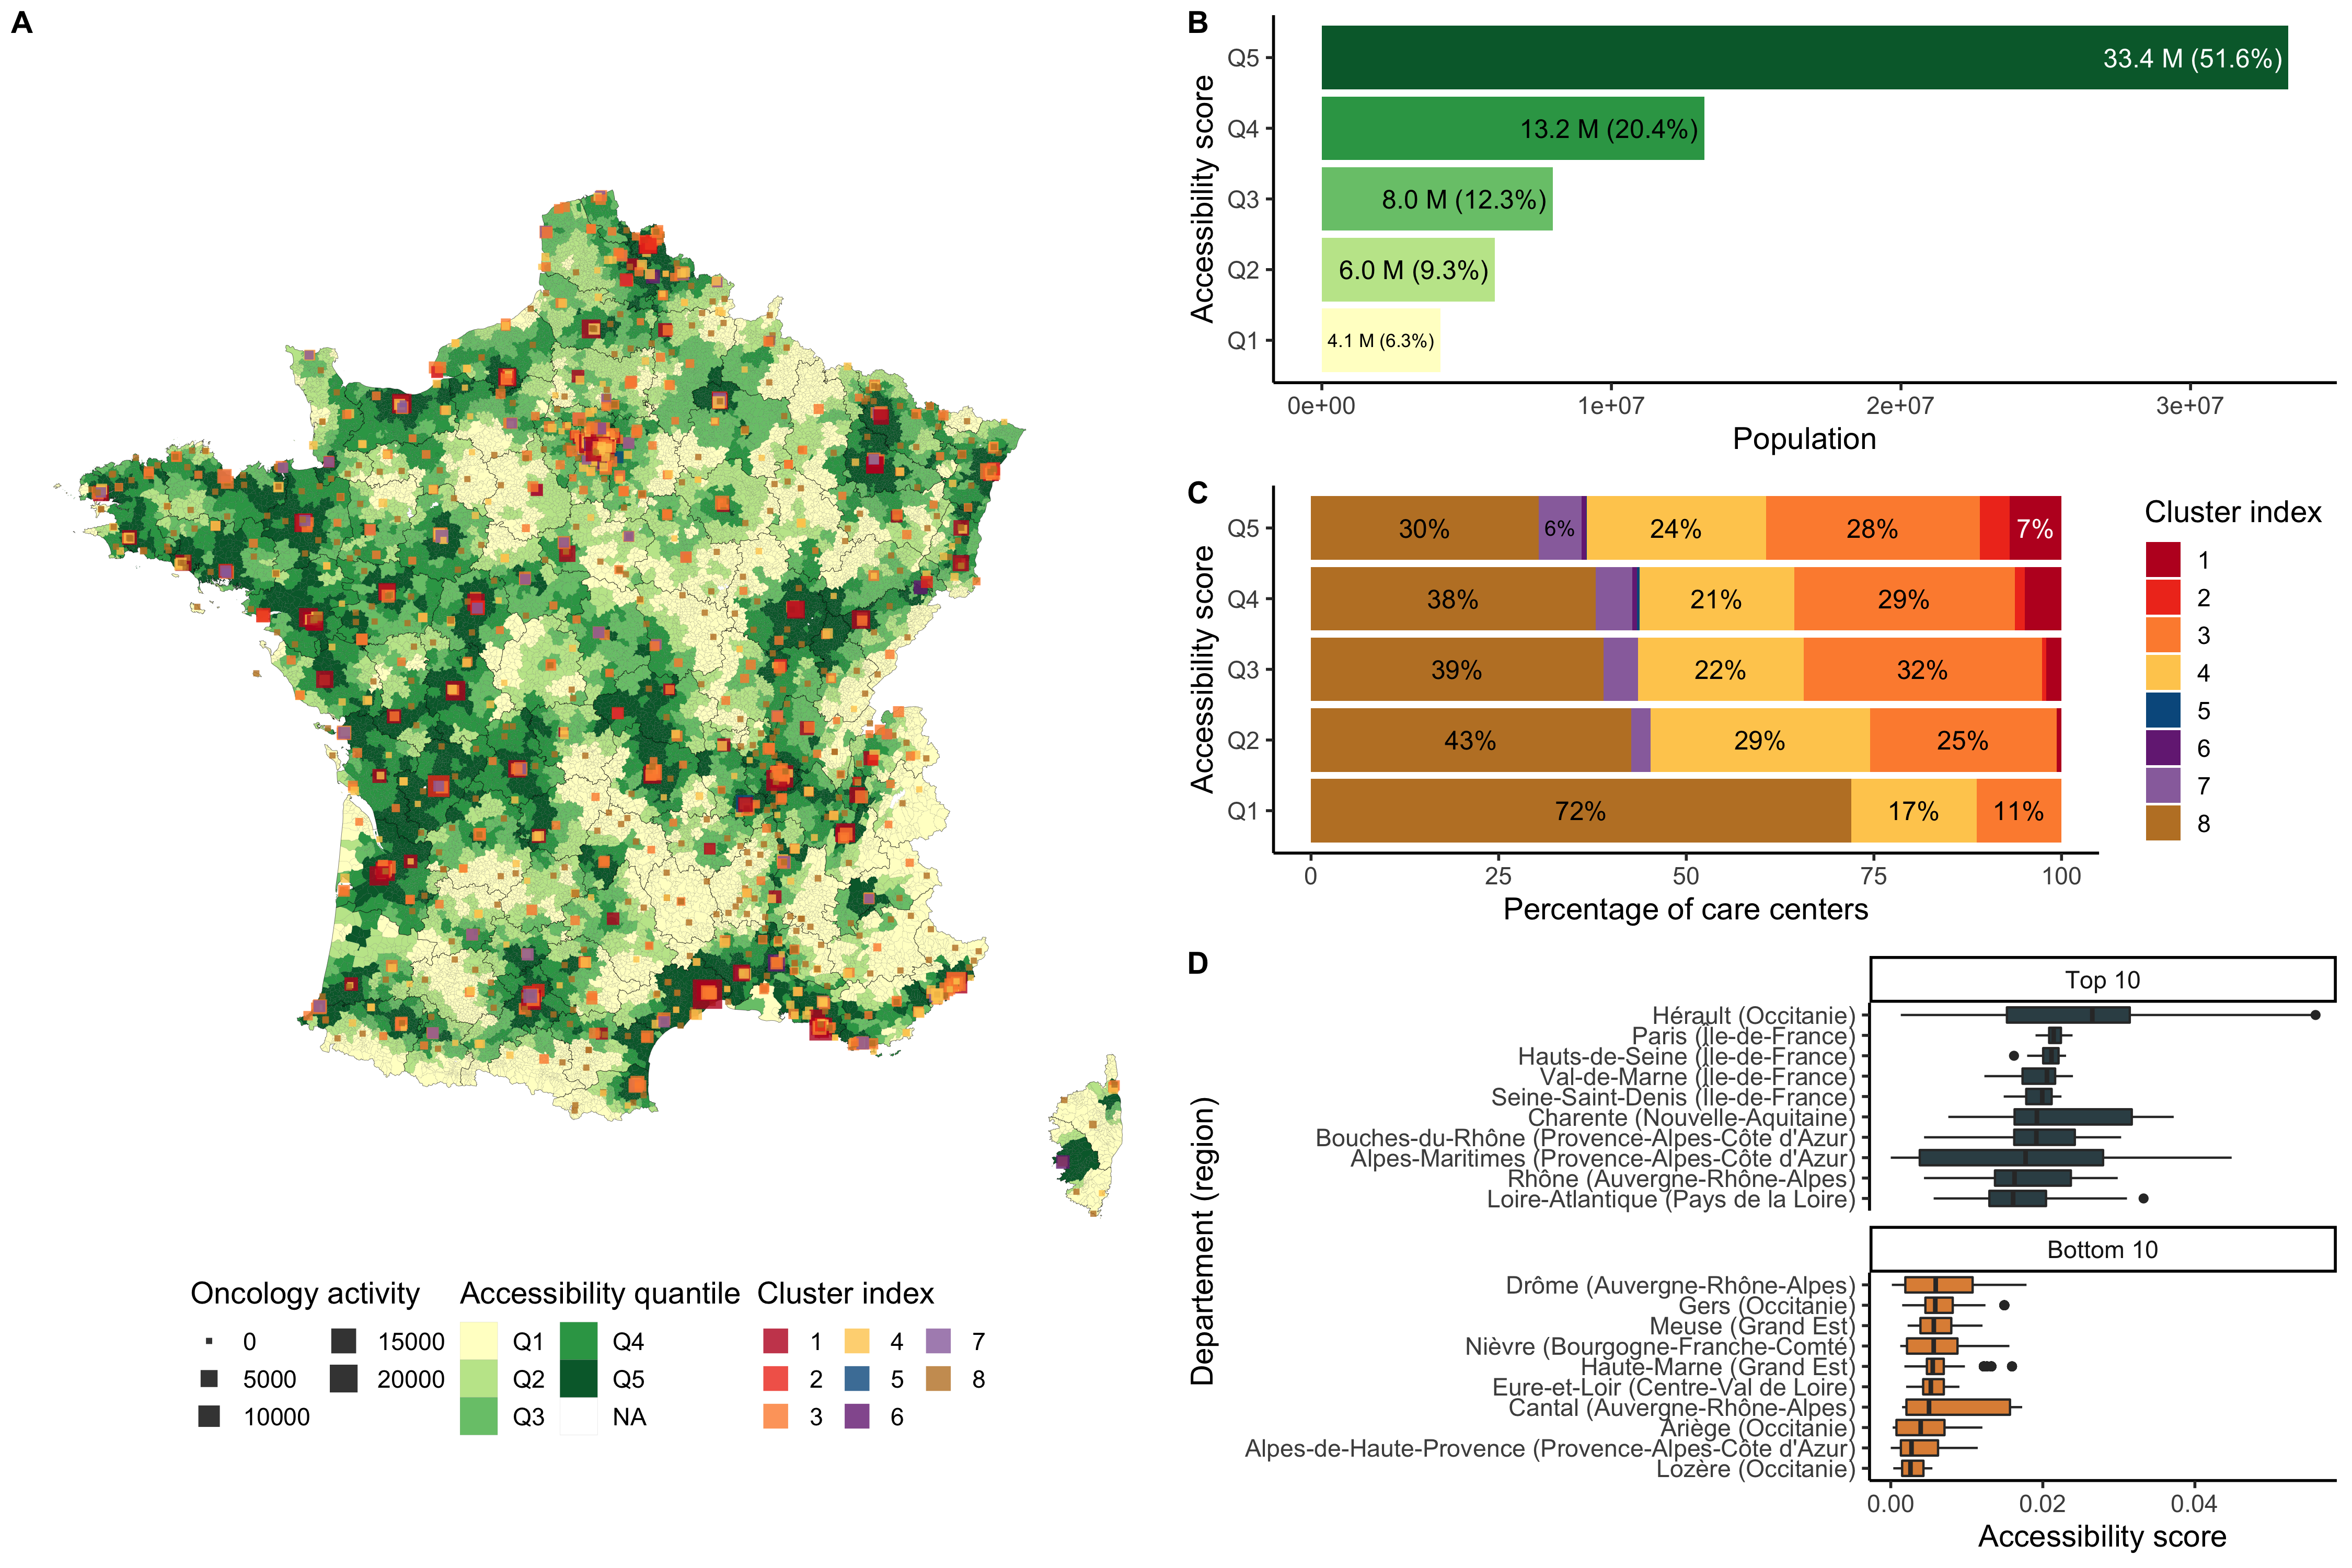
\includegraphics[width=0.9\textwidth]{images/camion/fig2_accessibility_france.png}
    \centering
    \caption{ \textbf{Distribution of the accessibility score computed with the
            \ac{e2sfca}, in metropolitan France.} Plot (A) shows municipalities
        colored by accessibility quantile. The care centers are drawn as
        squares, colored by cluster, and sized by oncology activity. Plot (B)
        shows the total population by accessibility quantile. Plot (C) displays
        the percentage of care centers by cluster by accessibility quantile.
        Plot (D) shows the top 10 and bottom 10 list of the departments, ranked
        by median accessibility. }
    \label{fig:accessibility-france}
\end{figure}

Accessibility score should be put into perspective with population density.
Overall, the denser municipalities have a median accessibility around 0.02.
Municipalities with low population densities have more extreme values.
\cref{fig:accessibility-vs-density} compares accessibility and population
density for three different regions: Provence-Alpes-Cote-d'Azur (A),
Ile-de-France (B), and Bourgogne-Franche-Comté (C). Municipalities are displayed
as squares, colored by accessibility quantile, and sized by population density.
These regions show very different profiles. In Provence-Alpes-Cote-d'Azur (A),
accessibility is essentially low in non-dense municipalities near the Alps.
However, in Bourgogne-Franche-Comté (C), we see dense municipalities with poor
accessibility scores, representing a large proportion of the region. We also
drew similar maps (D, E and F) where municipalities are colored based on the
average travel duration for patients with cancer in 2018. We see that the
average travel time is higher in municipalities with poor accessibility scores.

\begin{figure}[h!]
    \includegraphics[width=0.9\textwidth]{images/camion/fig3_accessibility_vs_density_scatter_map.png}
    \centering
    \caption{ \textbf{Comparison of population density with accessibility scores
            and patient average travel time for cancer pathways.} Showing results in
        three regions: Provence-Alpes-Cote-d'Azur (A, D), Ile-de-France (B, E)
        and Bourgogne-Franche-Comté (C, F). Municipalities are drawn as squares,
        sized by population density and colored by either accessibility quantile
        (A, B, C) or patient average travel time (D, E, F). }
    \label{fig:accessibility-vs-density}
\end{figure}

Finally, we compared our accessibility score with the department exit ratio, by
municipality. Department exit ratio is defined as the proportion of cancer
patients who visited a care center outside from their department of residence
and was computed using the \ac{pmsi} database. In Provence-Alpes-Cote-d'Azur,
the exit ratio is higher in departments with low accessibility scores and few
oncology specialized care centers, as in Alpes-de-Haute-Provence and
Hautes-Alpes. While the Var department has some oncology centers, exit ratio
remains high since larger care centers are in Marseille and Nice.

% \subsection{Accessibility distribution in metropolitan France regions}

\subsubsection{Accessibility in Provence-Alpes-Cote-d'Azur region}

We now focus on the region Provence-Alpes-Cote-d'Azur. This region is the far
southeastern on the mainland. The region's population was 5,048 million in 2018.
Its prefecture and largest city is Marseille. The region contains six
departments. Bouches-du-Rhone, Var and Alpes-Maritimes are located on the
coastline and gather the largest cities like Marseille, Nice, or Toulon.
Alpes-de-Haute-Provence, Vaucluse, and Hautes-Alpes are inland departments, with
a majority of rural and mountainous areas. Results are shown on
\cref{fig:accessibility-paca}. By comparing maps (A) and (B), we confirm that
the accessibility is maximum in denser areas of the region. Average patients
travel time are displayed on map (C) and we drew the major roads (primary,
motorway and truck) in red. The road system is well developed on the coast,
rallying the larger cities of the region. However, driving from the rural areas
in the Alps to the major cities is hard, resulting in higher travel times. The
accessibility is unevenly spread within the departments, especially in
Alpes-Maritimes where the distribution is multi-modal (D). There, cities like
Nice and Cannes have large hospitals thus good accessibility, while the northern
areas of the department are mostly mountains. Accessibility is higher in
municipalities with dense populations, for all the departments (E). Finally, the
average travel time decreases when the accessibility score increases. This makes
sense since the accessibility score was computed based on the driving distance
between population locations and care centers. However, it confirms that
patients living in poor accessibility zones effectively travel further to seek
oncology care. In Bouches-du-Rhone, nearly all the municipalities have an
average travel time lower than 30 minutes, while in Alpes-de-Haute-Provence,
average travel times are rarely lower than 60 minutes (F).

\begin{figure}[h!]
    \includegraphics[width=0.9\textwidth]{images/camion/fig4_accessibility_Provence-Alpes-Cote-d'Azur.png}
    \centering
    \caption{ \textbf{Accessibility distribution in Provence-Alpes-Cote-d'Azur
            region.} Map (A) shows the region accessibility distribution per
        municipality. Map (B) displays the population density discretized in 5
        bins. The map on plot (C) displays the average travel time for cancer
        pathways. Large roads (primary, motorway and trucks) are drawn in red.
        Plot (D) shows the accessibility distribution per department of the
        region. Plot (E) shows the accessibility distribution by municipality
        population density and department. Plot (F) compares the accessibility
        score from municipalities with the average travel time for cancer
        pathways. }
    \label{fig:accessibility-paca}
\end{figure}

\subsubsection{Accessibility in Pays de la Loire region}

The Pays de La Loire region is located in the west of France. It covers 32,082
km\textsuperscript{2} which makes it the largest region in France, with a
population of 3,806,461 (Insee) in 2019. In the region, one out of two
inhabitants lives in rural areas, compared to one out of three on average in
France. The Pays de la Loire is thus the 4th most rural region behind New
Aquitaine, Brittany and Burgundy-Franche-Comté.  The Pays de La Loire region is
composed of 5 departments. The level of population living in rural communes
varies according to the departments, but 4 departments out of the 5 are
considered rural.  In Vendée and Mayenne, two out of three inhabitants live in
rural areas, in Maine-et-Loire 58\% of the population resides in a rural commune
and in Sarthe 56\%. However, 29\% of the region's population lives in a rural
commune under the influence of a pole, compared to 20\% in an independent rural
commune. The city of Nantes, located in Loire-Atlantique in the east of the
region, is the largest urban area in the region and has 303,382 inhabitants, as
well as 961,521 inhabitants in its urban unit. The region has several cities
with more than 100,000 inhabitants with Le Mans and its 143,325 inhabitants,
Angers (151,520 inhabitants), followed by cities of about 50,000 inhabitants
such as Saint-Nazaire, (68,200 inhabitants) Cholet, (54,200 inhabitants) and
Laval (51,000 inhabitants). The Pays de la Loire has good accessibility with
51\% of its population living in a territory with maximum accessibility and a
low rate of its population living in territories with low or very low
accessibility: 8.3\% of its population resides in an accessibility score zone of
Q2 and only 3.7\% of its population in Q1. Thus, the maps show a good
distribution of accessibility across the territory that varies proportionally
with population density, with low accessibility areas corresponding to areas
with low or very low population density. Travel time is also relatively evenly
distributed across the region, with average travel times of 30 minutes, although
depending on the department, a significant proportion of trips are between 30
and 60 minutes. A very small proportion of territories exceed 60 minutes of
travel time. The territories with longer travel times are located in the Vendée
department, mainly due to the coastal profile of the department and the islands
that make it up, such as the Noirmoutier peninsula or the Ile d'Yeu, where
travel times exceed 90 minutes and 120 minutes respectively.

\begin{figure}[h!]
    \includegraphics[width=0.9\textwidth]{images/camion/region_accessibility/accessibility_Pays-de-la-Loire.png}
    \centering
    \caption{
        \textbf{Accessibility distribution in Pays-de-la-Loire.} The accessibility distribution
        in this region is high, and the amount of municipalities with Q5 accessibility
        score is very low. The median accessibility is the highest in Loire-Atlantique
        department, especially around Nantes; or in Maine-et-Loire near Angers. The
        lowest median accessibility is in Mayenne, where the main city is Laval. The
        accessibility is lower in the northern part of this department, where the
        population density decreases compared to the rest of the region.
    }
\end{figure}

\subsubsection{Accessibility in Occitanie region}

The Occitanie region is located in the South of France. It covers 72,724 km² for
a population of 5,933,185 (Insee) in 2019, for a population density of 81.6
inhabitants/km² the 6th least dense region in metropolitan France. The rural
territory in Occitanie represents 90\% of the territory, mainly present in the
mountain areas of the Massif Central and Pyrenees. The urban space is mainly
found along the coast and in the Garonne basin. 39\% of the population lives in
rural areas, i.e. 2.9 million inhabitants, and 9 of the 13 departments are
considered rural. However, Occitanie is a largely urbanized territory with
numerous urban centers in each department, the main metropolises being Toulouse
and Montpellier. This region is the 5th most urbanized region of the metropolis
and has more than fifty urban units of at least 10,000 inhabitants with several
cities exceeding 70,000 inhabitants (Tarbes, Montauban, Albi). 4.4 million
people live in the urban units, representing 76\% of the population. Occitanie
is composed of 13 departments. Three departments are among the most urbanized in
the province and therefore have a strong demographic weight: Hérault (89\% of
the population residing in an urban unit), Pyrénées-Orientales (88\%) and
Haute-Garonne (87\%). The Hérault department includes the city of Montpellier,
but also Béziers, Sète and many small urban areas. The Haute Garonne includes
the city of Toulouse, the fourth most populated commune in France (493,465
inhabitants) and with its rural areas are under strong pole influence.  The Lot,
Lozère and Gers are the least urbanized in France, with less than 40\% of the
population living in urban areas.

In this region, accessibility is not uniform across the territory. The areas
with the highest accessibility scores are concentrated in the large urban areas
and their catchment areas, notably in the center of the region around the city
of Toulouse and Montauban in the Garonne basin, as well as along the coastline
in the east of the region around the cities of Nîmes, Montpellier, Béziers,
Narbonne and Perpignan. Also, if the most densely populated areas have a good
level of accessibility, it can be seen that some medium-sized cities in the
Occitanie region lack a good level of accessibility and even have low
accessibility. This is particularly pronounced in the rural departments of the
region (Lot, Gers and Lozère), as well as in Aude, Ariège and Hautes-Pyrénées.
Indeed, many urban units have a low accessibility score (Q2) such as Auch
(25,527 inhabitants) in the Gers, Foix (12,310 inhabitants) and Pamiers (29,340
inhabitants) in the Ariège, Rodez (47,868 inhabitants) in the Aveyron with a
score of Q2/Q3, Cahors (24,279 inhabitants) in the Lot. Many areas of the region
have long travel times of around 90 minutes if not 120 minutes on average. This
is particularly true along the border with Spain, which is characterized by its
mountainous terrain. However, the Gers, Lot, Lozère, Aveyron and Hérault regions
have average travel times of around 90 minutes. These high travel times are
mainly associated with sparsely populated areas, although in the Hautes-Pyrénées
department, average travel times of 90 minutes can be seen around the urban unit
of Bagnères de Bigorre (13,213).

\begin{figure}[h!]
    \includegraphics[width=0.9\textwidth]{images/camion/region_accessibility/accessibility_Occitanie.png}
    \centering
    \caption{
        \textbf{Accessibility distribution in Occitanie.} The areas with the highest accessibility scores are concentrated in
        the large urban areas and their catchment areas, notably in the center of the
        region around the city of Toulouse and Montauban in the Garonne basin, as well
        as along the coastline in the east of the region around the cities of Nîmes,
        Montpellier, Béziers, Narbonne and Perpignan.
    }
\end{figure}

\subsubsection{Accessibility in Nouvelle-Aquitaine region}

The Nouvelle-Aquitaine region is located in the southwest of France. It covers
an area of 84,036 km\textsuperscript{2} which makes it the largest region in
France, with a population of 6,010,289 (Insee) in 2019. The region is the third
most rural region of France with half of its inhabitants living in a rural
commune. The share of population in rural autonomous is significant compared to
the national average but is similar to that of Brittany or
Burgundy-Franche-Comté. Among the twelve departments of Nouvelle-Aquitaine , ten
are predominantly rural, and two are predominantly urban: Gironde (71\% of the
population living in an urban commune) and Pyrénées-Atlantiques (62\%).
Nouvelle-Aquitaine is composed of 12 departments. The region's main metropolis,
Bordeaux, with 260,958 inhabitants and 986,879 inhabitants in its urban unit, is
located in the west of the region in the Gironde department. The region includes
several intermediate cities with more than 70,000 inhabitants such as Limoges
(130,876), Poitiers (89,212), Pau (75,627), La Rochelle (77,205), Mérignac
(72,197), Pessac (65,245).

We notice accessibility disparities in this region. The areas with the highest
accessibility scores are mainly located around the above-mentioned large and
intermediate cities. Also, the areas with accessibility scores Q1 and Q2 are
mainly located in territories with low or very low population density.
Similarly, the Nouvelle-Aquitaine region seems to provide relatively widespread
access to cancer care for its population. Indeed, 56\% of its population is
located in a zone with a maximum accessibility score of Q5, and 21.1\% in a zone
with a very good accessibility score of Q4. This leaves a smaller share of the
population in areas of low accessibility (8.4\% in Q2) and very low
accessibility (6.3\% in Q1). The average travel time is well distributed over
the territory, with a majority of the territory covered by travel times between
30 and 60 minutes. It can be seen, however, that part of the territory has a
good share of trips of less than 30 minutes (on average e 15 minutes) even in
areas with average accessibility (score 0.2). A clear correlation can be seen
between accessibility score and average travel time, with longer travel times in
areas with low accessibility scores, but consequently less densely populated
territories. The Landes and Lot-et-Garonne are the departments with the highest
number of trips exceeding 60 minutes.

\begin{figure}[h!]
    \includegraphics[width=0.9\textwidth]{images/camion/region_accessibility/accessibility_Nouvelle-Aquitaine.png}
    \centering
    \caption{
        \textbf{Accessibility distribution in Nouvelle-Aquitaine.}The areas with the highest accessibility scores are mainly located around the
        above-mentioned large and intermediate cities. Also, the areas with
        accessibility scores Q1 and Q2 are mainly located in territories with low or
        very low population density. The Nouvelle-Aquitaine region seems to
        provide relatively widespread access to cancer care for its population.
    }
\end{figure}

\subsubsection{Accessibility in Normandie region}

The Normandie region is located in the north-east of France. It covers 29,905
km² with a population of 3,325,032 inhabitants (Insee) in 2019. The Normandie
region remains a fairly rural region with half of its inhabitants living in a
rural commune (49\% compared to 40\% in the rest of France). The population
living in a rural commune is clearly in the majority in Orne in the south of the
region (73\%), Manche in the west (68\%) and Eure in the east (62\%). However,
more than half of the rural communes are not under the influence of a hub.
Normandie is composed of 5 departments. The department of Seine-Maritime in the
northeast of the region has two of the largest urban units in the region with
more than 200,000 inhabitants: Rouen the most populous with 112,321 inhabitants
and 471,893 in its urban unit as well as Le Havre with 172,366 inhabitants and
233,414 in its urban unit. The third urban unit of more than 200,000 inhabitants
in the region is Caen with 206,973 inhabitants in its urban unit, located in
Calvados. Normandie presents a rather average accessibility in terms of
population density and accessibility ratio since 30.9\% of its population lives
in the best accessibility score almost equivalent to the percentage of
population living in a territory with a Q3 score of 28.3\%. Only 10.3\% of its
population lives in accessibility level Q1 and 9.2\% in Q2.


We notice that the accessibility score is unevenly distributed. Although the
areas with low or very low population density are the most affected by a low
accessibility score of Q1 or Q2, we can still observe a fairly homogeneous
distribution of the population on the territory, especially in the areas far
from the urban units, and an accessibility that remains fairly low around Q2.
The department of Calvados has the best distribution of accessibility over its
entire surface. Whereas Orne, which is the most rural department in Normandie,
has an accessibility score of Q1 except around the urban unit of Argentant. The
same is true for the department of La Manche, which includes many areas of the
territory with an accessibility score of Q1 or especially Q2 despite a higher
population density, notably around the city of Cherbourg-Octeville and its
surroundings with an accessibility score of Q3 or even Q2 for a city that
nevertheless counts 35,545 and 81,423 in its urban unit (Figure 24). The average
travel time is well distributed over the territory, with the majority of the
territory covered by travel times of 30 minutes on average and below 60 minutes.
It can be seen that the majority of trips in the departments of Seine-Maritime
and Calvados are under 30 minutes, particularly in Calvados, unlike the
department of Orne, the only department in the region whose trips are slightly
over 60 minutes but still under 90 minutes.

\begin{figure}[h!]
    \includegraphics[width=0.9\textwidth]{images/camion/region_accessibility/accessibility_Normandie.png}
    \centering
    \caption{
        \textbf{Accessibility distribution in Normandie.}
    }
\end{figure}

\subsubsection{Accessibility in Île-de-France region}

The Île-de-France (IdF) region is located in the center north of France. This
one covers 12,012 km\textsuperscript{2} for a population of 12,213,447 (Insee)
in 2018. The IdF region is the most populated and dense of metropolitan France.
Only 5\% of the population lives in a rural commune, for the 671 rural communes
cover 59\% of the IdF territory. The majority of rural communes (85\%) are under
the influence of Paris. Île-de-France is composed of 8 departments, 4
departments in the inner suburbs and 4 departments in the outer suburbs. It is a
special region because it includes the French capital, Paris, the leading French
city in terms of demography and population density with 2,175,601 inhabitants in
2021. The city of Paris is also home to many specialized health establishments.
The rural communes are far from the influence of Paris and are mainly located in
the departments of the outer suburbs, three quarters of which are in
Seine-et-Marne. The most rural and least dense areas are therefore mainly
located in the east of the region, particularly along the border to the east of
the Seine-et-Marne department.

Île-de-France has good accessibility over the vast majority of its territory.
Indeed, 63.8\% of the population of IdF is located in an area with a maximum
accessibility score, and almost no population is located in an area with a
minimum accessibility score Q1 or even Q2. Also, although only 9\% of the
territory's surface is identified as having a Q5 score and 15\% as having a Q1
score, the minimum accessibility zones are not very densely populated, which
only affects a very small part of the region's population. Indeed, we observe
that the only areas with a Q1 score are located in the eastern part of the
region in the Seine-et-Marne department where the population density is very
low. Moreover, travel time is uniform throughout the region with a very good
level of travel time limited to an average of 30 minutes. The Ile-de-France
region does not suffer from accessibility difficulties at any level for cancer
treatments, regardless of location in the territory.

\begin{figure}[h!]
    \includegraphics[width=0.9\textwidth]{images/camion/region_accessibility/accessibility_Ile-de-France.png}
    \centering
    \caption{
        \textbf{Accessibility distribution in Ile-de-France.}Île-de-France has good accessibility over the vast majority of its territory.
        Indeed, 63.8\% of the population of IdF is located in an area with a maximum
        accessibility score, and almost no population is located in an area with a
        minimum accessibility score Q1 or even Q2. Also, although only 9\% of the
        territory's surface is identified as having a Q5 score and 15\% as having a Q1
        score, the minimum accessibility zones are not very densely populated, which
        only affects a very small part of the region's population.
    }
\end{figure}

\subsubsection{Accessibility in Hauts-de-France region}

The Hauts-de-France region is located in the north of France. It covers
31,948km² for a population of 6,005,000 (Insee) in 2019, or 9\% of the
metropolitan population. The region has retained a strong industrial footprint.
It is the second most urbanized region after Ile de France with 89\% of its
population living in a large urban area. However, 83\% of the region's
municipalities are considered rural (including autonomous rurality and rurality
under the influence of a pole in a peri-urban area), with 29\% of the region's
population living in a so-called rural municipality. The Hauts-de-France is
composed of 5 departments. In the department of Nord in the north of the region,
particularly urbanized and densified, is the city of Lille which has 1,411,571
inhabitants in its metropolis. Amiens in the department of Somme is the second
most populated urban area in the region.

The accessibility zones are relatively evenly distributed over the territory,
although the best accessibility in this department is mainly in the urban and
peri-urban area of Lille. Travel time averages 30 minutes over most of the
region, with the exception of the northern end of the region in the Aisne
department and the northeastern part of the same department, where travel time
averages 60 to 90 minutes. The population density is also low in these areas,
the Aisne being the least populated department in the Hauts-de-France region.
Only 4.4\% of the population of Hauts-de-France is located in an area with an
accessibility quantile of Q1 and 16.6\% in Q2. It is possible to perceive that
certain parts of the territory with a medium (100-200) to high (>200) population
density have an accessibility qualified at Q2 and Q3, which implies a difficulty
of accessibility of optimal care for certain segments of the population. In
fact, despite a low population rate in Q1, only 32.5\% of the regional
population is located in an area with the highest quantile of accessibility Q5.
These observations allow us to consider that the improvement of accessibility to
optimal care in this territory could be easily optimized because the initial
care offer is already well distributed in the territory with accessibility zones
Q4 and Q3, which together account for 46.4\% of the population.

\begin{figure}[h!]
    \includegraphics[width=0.9\textwidth]{images/camion/region_accessibility/accessibility_Hauts-de-France.png}
    \centering
    \caption{ \textbf{Accessibility distribution in Hauts-de-France.} The
        accessibility zones are relatively evenly distributed over the
        territory, although the best accessibility in this department is mainly
        in the urban and periurban area of Lille. Travel time averages 30
        minutes over most of the region, with the exception of the northern end
        of the region in the Aisne department and the northeastern part of the
        same department, where travel time averages 60 to 90 minutes }
\end{figure}

\subsubsection{Accessibility in Grand Est region}

The Grand Est region is located in the east of France. It covers 57,433
km\textsuperscript{2} for a population of 5,556,219 (Insee) in 2019. 39\% of the
population resides in a rural commune (i.e., a commune with low or very low
density). 61\% of the population resides in urban areas, 22.8\% in peri-urban
rural areas and 16.2\% in autonomous rural areas, moreover nearly 80\% of the
regional surface is dedicated to agriculture and forestry. The Grand Est is
composed of 8 departments. The departments of Meuse and Haute-Marne central to
the region are among the most rural departments in France with respectively 74\%
and 67\% of their population living in rural areas (peri-urban and autonomous),
while the departments of Haut-Rhin, Bas-Rhin, Meurthe-et-Moselle and Moselle
have more than 60\% of their population living in urban areas (2018, Insee). The
department of Marne in the west of the region is home to Reims, the most densely
populated city in the region after Strasbourg.

The accessibility is high in the eastern half of the region in the departments
of Moselle, Meurthe et Moselle, Bas-Rhin, Haut-Rhin, particularly around the
large agglomerations (Strasbourg, Nancy, Metz, Colmar). Indeed, 41\% of the
population of the Grand Est is in an accessibility zone of Q5 and only 7.5\% in
a Q1 zone. The lack of accessibility in the western part of the region is more
pronounced due to the low or very low density areas that are more common in
these departments. Also, the link between population density and accessibility
is visible and reinforced by the consideration of average travel times. Travel
times are almost uniformly distributed over the entire territory, with little or
no travel time exceeding 30 minutes; travel times of 60 minutes on average are
limited and those of 90 minutes are very limited. These times are most prevalent
in the western half of the region in the very low density areas but mostly in
the less demographically dense areas.  The poor accessibility for the city of
Charles-Ville-Mézière (46,436 inhabitants in 2019) is more worrying in view of
its demographic density. However, it can be observed that the coverage of
maximum accessibility for the majority of the population does not necessarily
require a spatial accessibility spread over the surface of the region, since the
Grand Est has only 13.5\% of the surface of its territory considered as Q5
accessibility, but covers the needs of maximum accessibility for 41\ of its
population. Thus, the urban nature of the population of the Grand Est seems to
be a determining factor in maximizing accessibility to care.

\begin{figure}[h!]
    \includegraphics[width=0.9\textwidth]{images/camion/region_accessibility/accessibility_Grand-Est.png}
    \centering
    \caption{ \textbf{Accessibility distribution in Grand-Est.} We notice good
        accessibility scores in the eastern half of the region in the
        departments of Moselle, Meurthe et Moselle, Bas-Rhin, Haut-Rhin,
        particularly around the large agglomerations (Strasbourg, Nancy, Metz,
        Colmar). Indeed, 41\% of the population of the Grand Est is in an
        accessibility zone of Q5 and only 7.5\% in a Q1 zone. The lack of
        accessibility in the western part of the region is more pronounced due
        to the low or very low density areas that are more common in these
        departments. }
\end{figure}

\subsubsection{Accessibility in Centre-Val de Loire region}

The Centre-Val-de-Loire region is located in the center west of France. It
covers an area of 39 151 km\textsuperscript{2} with a population of 2 573 180
(Insee) in 2019. The region is one of the most rural regions of France, with
90\% of its territory occupied by rural municipalities and 1 in 2 inhabitants
living in a rural municipality (49\%). 27\% of the population (700,000
inhabitants) live in a rural commune under the influence of a major pole and
nearly 22\% (of 570,000) outside the area of attraction of such a pole. However,
the CVdL includes two metropolitan areas, Orléans in the department of Loiret
and Tour in Indre-et-Loire, which together account for one-third of the regional
population. Paris also has an influence on the region, affecting 184,000
inhabitants under its influence, i.e., 7\% of the CVdL population. Thus, the
majority of the population (90\%) lives in an attractive urban area. The
Hauts-de-France is made up of 6 departments. The department of Indre-et-Loire
includes and Loiret includes the two metropolitan areas of the region Tour with
137,665 inhabitants and Orleans with 288,229 inhabitants in 2019.

The accessibility of the whole region is relatively lower than in other regions
observed so far. Many areas have a low or very low accessibility score despite a
medium population density. Areas with low or very low population density can
have a very low accessibility score, although low-density areas of the Cher have
a score around the Q3 quantile. Only the city of Tour and its vicinity shows a
maximum level of accessibility, as well as some surrounding parcel areas in the
department of Loir-et-Cher around the city of Blois and in the department of
Cher around Bourges. Even the city of Orleans has an accessibility score of Q4
despite the presence of level 1 clusters. The CVdL has the particularity of
being the only French region without a \ac{clcc} on its territory. The closest
\ac{clcc} are those in adjacent regions, in Paris in the Île-de-France and Anger
in Normandy. We can deduce that in order to access a specialized center, the
inhabitants of this region have to leave the region.  We can see that the level
1 clusters in the region are located in Tour, Orléans and Chartes. The
departments in the south of the region have lower level clusters, with the Cher
having only a level 3 and a level 7 cluster. This is reflected in the travel
times which are rather homogeneous and low in the northern and central
departments with average travel times of 30 minutes, while the southern
departments, Indre and Cher have much higher travel times throughout their
territory, around 60 minutes and 90 minutes.

\begin{figure}[h!]
    \includegraphics[width=0.9\textwidth]{images/camion/region_accessibility/accessibility_Centre-Val-de-Loire.png}
    \centering
    \caption{ \textbf{Accessibility distribution in Centre Val de Loire.} The
        accessibility of the whole region is relatively lower than in other
        regions observed so far. Many areas have a low or very low accessibility
        score despite a medium population density. Areas with low or very low
        population density can have a very low accessibility score, although
        low-density areas of the Cher have a score around the Q3 quantile. Only
        the city of Tour and its vicinity shows a maximum level of
        accessibility, as well as some surrounding parcel areas in the
        department of Loir-et-Cher around the city of Blois and in the
        department of Cher around Bourges. }
\end{figure}

\subsubsection{Accessibility in Bretagne region}

The region of Bretagne is located in the west of France, on the Atlantic coast.
It covers 27,208 km², making it the largest region in France, with a population
of 3,354,854 (Insee) in 2019. More than half of the Breton population (53.7\%)
resides in a rural commune, so Bretagne is the second most rural region of
metropolitan France after Burgundy-Franche-Comté. The Breton rural area is
characterized by longer travel times to everyday services. 25.7\% of the
inhabitants of very sparsely populated autonomous areas have to travel more than
10 minutes on average to access them, and for 68.6\% of them, the average
journey takes between 7 and 10 minutes. However, a major part of the population
lives in an attractive urban area, i.e. 87\% of the region's population.
Bretagne is composed of 5 departments. The main metropolis of the region is
Rennes with 215,366 inhabitants and 364,133 inhabitants in its urban unit, the
first agglomeration of the department of Ille-et-Vilaine, followed by Brest
which is located in the department of Finistère with 139,926 inhabitants.

Bretagne has very good accessibility with 57.7\% of its population living in a
territory with maximum accessibility and above all a very low rate of its
population in territories with low or very low accessibility with 5.1\% of its
population in Q2 and only 1.5\% of its population in Q1. Also, the maps show a
good distribution of accessibility throughout the territory, with variations
often related to the territory's population density ratio. Travel times reflect
the level of accessibility, with many travel times less than 30 minutes and some
travel times between 30 and 60 minutes but very rarely more. However, Morbihan
has a relatively high proportion of trips between 30 and 60 minutes, including
rare areas where travel times exceed 90 minutes, particularly due to the
department's profile, which includes certain islands such as Belle-Île, which
have travel times of over 120 minutes.


\begin{figure}[h!]
    \includegraphics[width=0.9\textwidth]{images/camion/region_accessibility/accessibility_Bretagne.png}
    \centering
    \caption{
        \textbf{Accessibility distribution in Bretagne.}
    }
\end{figure}

\subsubsection{Accessibility in Bourgogne-Franche-Comté region}

The Bourgogne-Franche-Comté (BFC) region is located in the center-east of
France. It covers 47,784 km\textsuperscript{2} for a population of 2,805,580
(Insee) in 2019 with 1,242,882 active people. In 2018 the BFC is considered the
first rural region of France with more than half of its population (1.5 million
people) residing in rural areas. The BFC is composed of 8 departments. The
departments of Yvonne, Nièvre to the west, Saône-et-Loire and Jura to the south,
have a particularly rural and agricultural landscape without dense urban areas,
especially for Saône-et-Loire.  In the department of Côte-d'Or is located Dijon,
the largest and most densely populated city in the region with 158,002
inhabitants, ahead of the city of Besançon with its 117,912 inhabitants, which
is located to the east in the department of Doub. In total, the BFC region has
3,704 municipalities, 26 of which have more than 10,000 inhabitants.

The departments of Côte-d'Or and Doubs have the best accessibility, especially
around densely populated urban areas such as Dijon or Besançon. Some areas of
the region have a low accessibility quantile Q1 and Q2 which cover 37.3\% and
16.4\% respectively of the regional territory, i.e. more than half (53.7\%) of
the area is recognized with a level of accessibility to cancer care. The areas
with low or very low accessibility are located mainly in rural areas and with
low or very low population density, except for the eastern border of the Doubs,
which has more densely populated areas, but with more mountainous terrain, with
a quantile 1 accessibility. In each department, accessibility is best in the
urban areas and their surroundings. The travel time shows an unequal
distribution of access to health care in the territory, since the majority of
municipalities have an average travel time of 30 minutes, but large areas of the
region show average travel times of 60 or 90 minutes, particularly in the
departments of Nièvre and Yvonne, although in the less densely populated areas
of these departments, or travel times exceeding 120 minutes in the east of the
Jura at the Swiss border, which is, however, likely to be a more mountainous
terrain

\begin{figure}[h!]
    \includegraphics[width=0.9\textwidth]{images/camion/region_accessibility/accessibility_Bourgogne-Franche-Comte.png}
    \centering
    \caption{ \textbf{Accessibility distribution in Bourgogne-Franche-Comté.}
        The departments of Côte-d'Or and Doubs have the best accessibility,
        especially around densely populated urban areas such as Dijon or
        Besançon. Some areas of the region have a low accessibility quantile Q1
        and Q2 which cover 37.3\% and 16.4\% respectively of the regional
        territory, i.e. more than half (53.7\%) of the area is recognized with a
        level of accessibility to cancer care. The areas with low or very low
        accessibility are located mainly in rural areas and with low or very low
        population density, except for the eastern border of the Doubs, which
        has more densely populated areas, but with more mountainous terrain,
        with a quantile 1 accessibility. }
\end{figure}

\subsubsection{Accessibility in Auvergne-Rhône-Alpes region}

The Auvergne-Rhône-Alpes (ARA) region is located in eastern France. It covers
69,711 km\textsuperscript{2} for a population of 7,994,459 (Insee) in 2018,
representing 12.3\% of the metropolitan population, i.e. the most populated
region in France. The ARA is the main mountain region of France with 2.2 million
people residing in a municipality classified as a mountain area, with more than
half in the regional part of the Massif Central which is distributed in a
diagonal of low population density, while the population of the Alpine massif is
concentrated in the urbanized and more densely populated parts at the bottom of
valleys. In the ARA, 35\% of the population lives in a rural commune, the
provincial metropolitan average being 33\%, and these communes cover 89\% of the
region's surface area. The ARA is composed of 12 departments. The Rhône
department in the northern center of the region includes the city of Lyon, the
second largest city in France, which has 1,411,571 inhabitants in its
metropolis. The eastern departments, Savoie, Haute-Savoie, Isère, Drôme,
constitute the mountainous areas of the region. Of the twelve departments, five
are considered 'essentially rural': Cantal (74\% of the inhabitants live in
rural communes), Haute-Loire (70\%), Ardèche (60\%), Allier (58\%) and Ain
(50\%).

If we look at the maps, we can see that the areas with the lowest accessibility
are mainly located in areas with low or very low density, particularly along the
mountainous border in the east of the region in the departments of Haute-Savoie,
Savoie, Isère and Drôme. It is possible to observe a good distribution of
accessibility in the central, northern and north-western part of the region,
particularly around the large agglomerations such as the city of Lyon,
Clermont-Ferrand, Moulins, Grenoble and Aurillac. The three southern
departments, Haute-Loire, Ardèche and Drôme, are less accessible than the other
departments in the region. Above all, it can be observed that the mountainous
terrain tends to have a strong impact on accessibility to care, since travel
times in these areas, particularly for the departments of Drôme and Savoie,
reach an average of 120 minutes if not 150 minutes. In the mountainous
departments of the east, the valleys that contain the urban centers with the
highest population density, such as Chambéry, Grenoble and Annecy, are the most
favorable accessibility centers in these departments. Despite its mountainous
nature, 51.1\% of the Auvergne-Rhône-Alpes region is located in an accessibility
zone Q5 compared to 8\% in an accessibility zone Q1.

\begin{figure}[h!]
    \includegraphics[width=0.9\textwidth]{images/camion/region_accessibility/accessibility_Auvergne-Rhone-Alpes.png}
    \centering
    \caption{ \textbf{Accessibility distribution in Auvergne-Rhone-Alpes.} The
        areas with the lowest accessibility are mainly located in areas with low
        or very low density, particularly along the mountainous border in the
        east of the region in the departments of Haute-Savoie, Savoie, Isère and
        Drôme. It is possible to observe a good distribution of accessibility in
        the central, northern and north-western part of the region, particularly
        around the large agglomerations such as the city of Lyon,
        Clermont-Ferrand, Moulins, Grenoble and Aurillac. The three southern
        departments, Haute-Loire, Ardèche and Drôme, are less accessible than
        the other departments in the region. Above all, it can be observed that
        the mountainous terrain tends to have a strong impact on accessibility
        to care, since travel times in these areas, particularly for the
        departments of Drôme and Savoie, reach an average of 120 minutes if not
        150 minutes. }
\end{figure}

\section{Conclusion}

In this section, we described our method to compute the oncology accessibility
score given to every municipality in metropolitan France. This score was
obtained by using the \acf{e2sfca} algorithm, with oncology activity as supply,
municipality population as demand, and driving car duration as impedance metric.
Specific attention should be given to municipalities with very poor access to
oncology care centers. While we saw that most of the population lives in high
accessibility areas, around 6\% of the population lives in the bottom 20\%
accessibility quantile. Among these municipalities, some are very rural and
mountainous like those in the Alpes-de-Haute-Provence in
Provence-Alpes-Cote-d'Azur region. Such areas cannot be expected to have a very
good healthcare coverage. By contrast, the case of suburban areas with
relatively dense population and poor accessibility should be addressed more
easily. Our optimization algorithm can help driving public health policies, as
it effectively identifies areas where accessibility could grow, by allocating
additional oncology activity to a restricted number of care centers. The
proposed growth factors are indicative and do not have to be effective within a
year, as it represents a considerable effort for care centers to increase their
activity. Our oncology accessibility score is deliberately non-specific to
cancer type. This score is meant to outline how easy it would be for a
population location to reach a first entry point for oncology care. Here, we are
only focusing on surgery, chemotherapy, and radiotherapy treatments. The same
technique could be used on a specific cancer type, the method will remain the
same, only the supply variable used in the accessibility score will change. We
should mention that \ac{sa} is better suited for pathologies that are relatively
well handled across the whole country. Accessibility for rare diseases like
pediatric cancer or complex cancers that re-quire a specific expertise is less
informative because only a handful of care centers are indicated. Similarly, we
could compute an accessibility score that is focused on specific kinds of stays:
our web application lets the user pick between surgery, chemotherapy, or
radiotherapy as supply variable.

\chapter{\acf{camion}}

\section{Motivation}

Uneven distributions of population and health-care providers lead to geographic
disparity in accessibility for patients \cite{wang_why_2020}, illustrated by our
previous results on accessibility. Several methods have been developed to
address these disparities. Location-allocation algorithms
\cite{church_location_1999} can optimize the distribution and supply of health
providers to reduce accessibility disparities. These algorithms seek the optimal
placement of facilities for a desirable objective under certain constraints
\cite{wang_measurement_2012}. For instance, an optimization algorithm  was
developed to improve the healthcare planning in rural China by finding the best
place and capacity for new health facilities \cite{luo_integrating_2014}.
A spatial optimization model was designed to maximize equity in accessibility
to residential care facility in Beijing, China \cite{tao_spatial_2014}. When
optimizing health accessibility, there are two competing goals: equity and
efficiency \cite{krugman_opinion_2013,meyer_equity_2008}. Equity may be defined
as equal access to healthcare for everyone \cite{culyer_equity_1993}. An
efficient situation is when everything has been done to help any person without
harming anyone else \cite{hemenway_optimal_1982}. While some argue that
efficiency should be ad-dressed in priority \cite{hemenway_optimal_1982}, others
agree that equity is a matter of ethical obligation, especially in public health
\cite{fried_rights_1975, oliver_equity_2004}. Regarding efficiency optimization,
the most popular algorithms are p-median, \ac{lscp} and \ac{mclp}. The p-median
algorithm minimizes the weighted sum of distances between users and facilities
\cite{murad_using_2021}. \ac{lscp} minimizes the number of facilities needed to
cover all demand \cite{shavandi_fuzzy_2006}. \ac{lscp} maximizes the demand
covered within a desired distance or time threshold by locating a given number
of facilities \cite{casado_heuristical_2005}. To reach equal access to
healthcare, quadratic programming has been used to  minimize the variance of
accessibility scores defined by the \ac{2sfca} \cite{wang_planning_2013}.
Similarly, a \ac{pso} algorithm was developed to minimize the total square
difference between the accessibility score of each demand location and the
weighted average accessibility score \cite{tao_spatial_2014}. Finally, a
two-step optimization algorithm has been developed to address the dual
objectives of efficiency and equality, by first choosing where to site new
hospitals and then deciding which capacity they should have
\cite{luo_two-step_2017,li_two-step_2017}.

However, most of the previous algorithms seek locations to open new health
facilities. Regarding oncology care, opening new facilities can be very costly
and hard in practice. In this work, we are interested in the case where the
health facilities locations are fixed, and the only lever to improve
accessibility is to increase their capacities.Given a capacity budget, we want
to know which facilities to grow and by how much. We introduce \ac{camion}, an
accessibility optimization algorithm based on \ac{fca} and \ac{lp}. The initial
accessibility score was computed with the \ac{e2sfca} algorithm
\cite{luo_enhanced_2009} but our algorithm can generalize to more \ac{fca}
derivatives. In the following sections, we proposed two approaches for
optimizing the accessibility scores. The first one is an overall optimization,
where we seek to maximize the total accessibility. The second one is a maxi-min
optimization, where we want to maximize the minimum accessibility instead. The
first approach could be seen as efficiency maximization where the second method
aims towards equity. Then, we embedded our results and algorithms into a
web application  called ``oncology-accessibility''. Through this web
application, we let the users run the optimization algorithm with the
parameters they want, and visualize the output on interactive maps and
figures. We believe such an app could benefit the healthcare professionals,
to help addressing the accessibility disparities in the country.

\section{Methods}

\subsection{Overall optimization}

We model the problem as an optimization task. In our case, we want our
optimization algorithm to find new care centers capacities given some
constraints, so that the total accessibility is maximum. We apply optimization
on a given region only, rather than on the whole metropolitan France. We chose
this approach because healthcare planning is handled regionally rather than
nationally. We show below that our optimization problem is a \acf{lp} problem. In
its standard form, \ac{lp} finds a vector $x$ that maximizes $c^T x$ under
constraints $Ax \leq b$, where $A$ is a matrix and $b$ a vector. Boundaries can
be set to $x$ such as $x \geq 0$. Consider $x_u$ the new capacity of a care
center $u$, to be computed by the algorithm. Let $Q_u$ and $W_u$ be two vectors
of size $m$, defined as follows:

\begin{align}
    Q_u & =  \sum_{s=1}^{r} W_s \sum_{i, d_{iu} \in I_s} P_i \\[10pt]
    W_u & =  \sum_{s=1}^{r} \sum_{i, d_{iu} \in I_s} W_s
\end{align}

Intuitively, $Q_u$ is the weighted population that has access to the care center
$u$, and $W_u$ is the sum of weights of municipalities that have access to $u$.
We can compute the total accessibility as a sum on the $m$ care centers:

\begin{align*}
    \sum_{i} A_i & = \sum_{i} \sum_{s=1}^{r} W_s \sum_{u, d_{iu} \in I_s} \frac{S_u}{Q_u} \\[10pt]
    \sum_{i} A_i & = \sum_{i} \sum_{i, d_{iu} \in I_s} W_s \frac{S_u}{Q_u}                \\[10pt]
    \sum_{i} A_i & = \sum_{u} \frac{S_u}{Q_u} \sum_{s} \sum_{i, d_{iu}} W_s               \\[10pt]
    \sum_{i} A_i & = \sum_{u} \frac{S_u}{Q_u} W_u \numberthis \label{eq:A_i_sum_u}
\end{align*}

\cref{eq:A_i_sum_u} can be rewritten in the \ac{lp} standard form with:

\begin{align*}
    c                & = \frac{W_u}{Q_u}              \\
    x_u              & = S_u                          \\
    b                & \geq \sum_{u} x_u              \\
    x_{u_\text{min}} & \leq x_u \leq x_{u_\text{max}}
\end{align*}

The user-defined parameters are $b$, $x_{u_\text{min}}$ and $x_{u_\text{max}}$.
$b$ is the total capacity to be shared across all the care centers.
$x_{u_\text{min}}$ and $x_{u_\text{max}}$ are the capacity boundaries for care
center $u$. If $b$ is set to the current total capacity, a care center can’t be
grown unless another one is decreased. If $b > \sum_{u} x_u$, the capacity of
care centers can be increased without decreasing other centers. We know how to
solve \ac{lp} and we used the SciPy \cite{virtanen_scipy_2020} implementation of
the revised simplex method as explained in \cite{bertsimas_introduction_1998}.
We now detail how we set the user-defined parameters to apply the \ac{lp}
algorithm to our specific case. The additional capacity was set as +3\% of the
overall activity of the region's care centers: $b = 1.03 \times \sum_{u} x_u$.
The choice of the boundaries $x_{u_\text{min}}$  and $x_{u_\text{max}}$ is
crucial and must be realistic. We studied the hospitals activity on the past
four years (2016 to 2019) to retrieve the average growth percentage of a care
center. The growth percentage is computed as follows: $(S_\text{2019} -
    S_\text{2016}) / S_\text{2016}$ . Among the care centers that grew and who had
an existing oncology activity, the mean growth percentage was 23\%. Hence, we
set $x_{u_\text{max}}$ as +20\% of the care center capacity. Regarding
$x_{u_\text{min}}$, we set the boundary based on the cluster of the care center.
For the three most specialized clusters, we set their $x_{u_\text{min}}$ equal
to their current activity. We did this to prevent the algorithm from decreasing
the most specialized and well-equipped care centers. Regarding the care centers
from the other clusters, $x_{u_\text{min}}$, so that they could be emptied if
need be. Finally, we set $x_{u_\text{max}}$ if the care center belongs to the
least specialized cluster. The new capacities are indicative and should be
further investigated to make sure they are relevant. Especially when setting an
existing oncology activity to 0.

\subsection{Maxi-min optimization}

We now want to maximize the minimum accessibility, meaning that the facilities
capacities will be increased to develop the areas where the accessibility is
minimum in priority. Let $z$ be the minimum accessibility score.

\begin{align}
    z & = \underset{i=1, ..., n}{min} A_i       \\
    z & \leq A_i \; \text{for all} \; i=1,...,n
    \label{eq:z-inequality}
\end{align}

Let $x_u$ be the capacity increase for facility $u$,
whose current capacity was $S_u$. A facility with an unchanged capacity will
have $x_u=0$. The accessibility score $A_i$ at municipality $i$ computed with the
\ac{e2sfca} algorithm can be written as:

\begin{align*}
    A_i & = \sum_{s=1}^{r} W_s \sum_{u,d_{iu} \in I_s} \frac{S_u + x_u}{Q_u}
    \label{eq:A_i}
\end{align*}

Replacing $A_i$ with this previous formulation in \cref{eq:z-inequality} brings
the following:

For all $i=1, ... ,n$:

\begin{align*}
    z                                                              & \leq \sum_{s=1}^{r} W_s \sum_{u, d_{iu} \in I_s} \frac{S_u + x_u}{Q_u} \\
    z - \sum_{s=1}^{r} W_s \sum_{u,d_{iu} \in I_s} \frac{x_u}{Q_u} & \leq \sum_{s=1}^{r} W_s \sum_{u,d_{iu} \in I_s} \frac{S_u}{Q_u}
\end{align*}

We can add these new $n$ equations as constraints to the optimization problem,
as well as the other constraints. The Linear Programming problem is now framed
as the maximization of $c^T x$ with $c=(1, ... ,0)$ and $x=(z, ... ,0)$, both of
size $m+1$ with m the number of facilities. The constraints are:

For all $i=1, ... ,n$:

\begin{align*}
    z - \sum_{s=1}^{r} W_s \sum_{u,d_{iu} \in I_s} \frac{x_u}{Q_u} & \leq \sum_{s=1}^{r} W_s \sum_{u,d_{iu} \in I_s} \frac{S_u}{Q_u} \\
    \sum_{u} x_u                                                   & \leq b \; \text{for a given budget} \; b                        \\
    x_{u_\text{min}}                                               & \leq x_u \leq x_{u_\text{max}}
\end{align*}

\section{Results}

We now present the outcomes of our optimization algorithm, on every region in
metropolitan France. We chose to run the overall optimization approach, because
it led to better results. Indeed, with the maxi-min approach, the municipalities
with low population densities and few hospitals were targeted first. Since these
municipalities often have access to non specialized hospitals, the only lever we
had was to develop these smaller hospitals, which could be very costly. The
algorithm was ran on every region and the additional number of stays was set to
3\% of the current region's overall activity and capped care centers to a
20\% maximum growth.

\subsection{Optimization results in metropolitan France regions}

\subsubsection{Provence Alpes Cote d'Azur}

We allocated 3,221 new stays in this region, corresponding to 3\% of the overall
activity. The median accessibility in the region went from 0.0093 to 0.0103, a
11.1\% increase. The results are shown on \cref{fig:optim-paca}. Map (A)
displays the accessibility delta ($A_{i_\text{after}} - A_{i_\text{before}}$) as
well as the care centers eligible to grow. Centers from cluster 8 were hidden
since we considered that they couldn't provide any oncology activity. The
algorithm identified a list of 26 care centers where the oncology activity could
grow to maximize the total accessibility in the region. These centers are either
public or private hospitals, primarily located in the Avignon and Gap areas. The
care centers located in high accessibility areas near Marseille and Nice were
ignored by the algorithm because improving these zones is not a priority. The
care center that grew the most is Clinique Sainte Catherine, in Avignon.
Interestingly, this care center was recently bought by the Unicancer group,
which coordinates all the cancer centers in France. This hospital's type will
change to become a new \ac{clcc}. Thus, it is expected to grow in the next years
and to be equipped with more oncology services and staff.

\begin{figure}[h!]
    \includegraphics[width=0.9\textwidth]{images/camion/fig5_Provence-Alpes-Cote-d'Azur.png}
    \centering
    \caption{ \textbf{Accessibility delta in Provence-Alpes-Cote-d'Azur region
        after running the optimization algorithm.} Map (A) displays the
    accessibility delta ($A_{i_\text{after}} - A_{i_\text{before}}$) by
    municipality. Plot (B) shows the capacity delta
    ($S_{u_\text{after}}-S_{u_\text{before}}$) distribution. Capacity was
    defined as the oncology activity: the number of patients with
    chemotherapy or radiotherapy and the number of medical or surgery stays
    related to oncology. We show the list of the care centers that grew the
    most (C)  and by how much. For instance, the hospital Institut Sainte
    Catherine in Avignon, was assigned a +1,030 capacity, for a total of
    n=6,179. Additional activity was 3,221. 26 centers grew and 1 decreased.
    Median accessibility before optimization was 0.0093 and 0.0103 after,
    corresponding to a 11.1\% increase.  Accessibility increased around
    cities like Avignon and Gap. Care centers near Nice were left unchanged
    by the algorithm. }
    \label{fig:optim-paca}
\end{figure}

\subsubsection{Pays de la Loire}

Similarly, we describe the optimization results in the Pays-de-la-Loire region,
obtained with the same parameters for the algorithm. The additional activity was
1,890. A total of 18 centers grew and 2 were decreased. The median accessibility
before optimization was 0.0118 and 0.0121 after, corresponding to a 2.4\%
increase. Accessibility mainly grew near Le Mans, Angers and La Roche sur Yon.
The three hospitals that had the highest increase in capacity were \ac{ch}
du Mans, a public hospital; Clinique Victor Hugo, a private hospital; and
Centre Jean Bernard, a private hospital dedicated to oncology and located
right next to Clinique Victor Hugo. Developing these areas will benefit patients
living there and prevent them to travel to Nantes, Rennes or Angers when it is
not necessary, thus avoiding long drives.

\begin{figure}[h!]
    \includegraphics[width=0.9\textwidth]{images/camion/optim_region/optim_Pays-de-la-Loire.png}
    \centering
    \caption{ \textbf{Optimization results in Pays-de-la-Loire.} Additional
        activity was 1,890. 18 centers grew and 2 decreased. Median
        accessibility before optimization was 0.0118 and 0.0121 after,
        corresponding to a 2.4\% increase. Accessibility mainly grew near Le
        Mans, Angers and La Roche sur Yon. }
\end{figure}

\subsubsection{Occitanie}

In Occitanie, the additional activity was 3,652. 28 centers grew and 1
decreased. Median accessibility before optimization was 0.0087 and 0.0091 after,
corresponding to a 4.7\% increase. Accessibility mainly grew around Perpignan,
Rodez, Mende and Tarbes. The two largest cities in the region Toulouse and
Montpellier were ignored by the algorithm, since this is where the largest
hospitals already are. The three hospitals that were the most developed by the
algorithm are Clinique Saint Pierre, a private hospital; \ac{ch} Perpignan
which is public and Centre Catalan d'Oncologie Saint Pierre, a private
hospital dedicated to oncology located in Perpignan. The three areas picked
by the algorithm are located apart from each other on the outskirts
of the region.

\begin{figure}[h!]
    \includegraphics[width=0.9\textwidth]{images/camion/optim_region/optim_Occitanie.png}
    \centering
    \caption{ \textbf{Optimization results in Occitanie.} Additional activity
        was 3,652. 28 centers grew and 1 decreased. Median accessibility before
        optimization was 0.0087 and 0.0091 after, corresponding to a 4.7\%
        increase. Accessibility grew around Perpignan, Rodez, Mende and Tarbes.
    }
\end{figure}

\subsubsection{Nouvelle-Aquitaine}

In Nouvelle Aquitaine, the additional activity was 3,445. A total of 25 centers
grew and 1 decreased. The median accessibility before optimization was 0.0117 and
0.0119 after, corresponding to a 1.5\% increase. Accessibility mainly grew around
Limoges, Angoulême, and Brive-la-Gaillarde. Unlike in the Occitanie region,
the algorithm picked areas that are fairly close to each others, mostly located
on the northern east part of the region. The largest city Bordeaux was again
left unchanged by the algorithm. The three hospitals with the largest increase
in capacity are \ac{chru} Dupuytren in Limoges; \ac{ch} Dubois in
Brive-la-Gaillarde and Clinique François Chenieux in Limoges.

\begin{figure}[h!]
    \includegraphics[width=0.9\textwidth]{images/camion/optim_region/optim_Nouvelle-Aquitaine.png}
    \centering
    \caption{ \textbf{Optimization results in Nouvelle-Aquitaine.} Additional
        activity was 3,445. 25 centers grew and 1 decreased. Median
        accessibility before optimization was 0.0117 and 0.0119 after,
        corresponding to a 1.5\% increase. Accessibility grew around Limoges,
        Angouleme, and Brive-la-Gaillarde. }
\end{figure}

\subsubsection{Normandie}

In Normandie, the additional activity was 1,523. A total of 15 centers grew and
none decreased. The median accessibility before optimization was 0.0105 and 0.0106 after,
corresponding to a 1\% increase. Accessibility mostly grew near Caen, Argentan, and
St-Lo, on the middle-western part of the region. Hospitals near Rouen and Évreux
were left unchanged by the optimization process. The algorithm mostly targeted
a single hospital: the \ac{chru} Cote de Nacre, a public university hospital in
Caen. This hospital received a +771 activity, for a total of 4628 stays. The
other hospitals that were increased are smaller, and their number of stays
range between 24 and 725.

\begin{figure}[h!]
    \includegraphics[width=0.9\textwidth]{images/camion/optim_region/optim_Normandie.png}
    \centering
    \caption{ \textbf{Optimization results in Normandie.} Additional activity
        was 1,523. 15 centers grew and 0 decreased. Median accessibility before
        optimization was 0.0105 and 0.0106 after, corresponding to a 1\%
        increase. Accessibility grew near Caen, Argentan, and St-Lo. }
\end{figure}

\subsubsection{Île-de-France}

In Ile-de-France, the additional activity was 5,826. 44 centers grew and 1
decreased. The median accessibility before optimization was 0.0088 and
0.0089 after, corresponding to a 1.3\% increase. Accessibility grew
around Mantes-la-Jolie, Rambouillet, Melun, and Évry, on the outskirt of the
region, surrounding the Paris city. Looking at the map, it is harder to
distinguish specific areas that were developed, since the accessibility
increase is much more spread than in the other regions. This is probably
due to the relatively high population densities in the whole region. Developing
the hospitals outside of the Paris city seems fair, given the tedious drive
that it would take to reach the city center from the suburbs, especially due to
the traffic. Moreover, the most specialized hospitals in Paris are often
already saturated, from patients living in Paris or coming from other regions
in the case of rare cancers.

\begin{figure}[h!]
    \includegraphics[width=0.9\textwidth]{images/camion/optim_region/optim_Ile-de-France.png}
    \centering
    \caption{ \textbf{Optimization results in Ile-de-France.} Additional
        activity was 5,826. 44 centers grew and 1 decreased. Median
        accessibility before optimization was 0.0088 and 0.0089 after,
        corresponding to a 1.3\% increase. Accessibility grew around
        Mantes-la-Jolie, Rambouillet, Melun, and Évry. }
\end{figure}

\subsubsection{Hauts-de-France}

In Hauts-de-France, the additional activity was 2,520. A total of 29 centers
grew and 1 decreased. The median accessibility before optimization was 0.01 and
0.0102 after, corresponding to a 2.1\% increase. Accessibility mainly grew
around St-Quentin and Valenciennes. Similarly to the results in Ile-de-France
region, it is relatively hard to distinguish precise areas where the accessibility
was increased, and the accessibility delta is more evenly spread around the region.
However there are areas where the hospitals remained unchanged, in Lille for instance or
in the southern part of the region, in the Oise department, near Beauvais,
Compiègne or Senlis. The two hospitals where the capacity increase were the
largest are Centre Leonard de Vinci, a private structure near Douai; \ac{ch}
Saint Quentin, a public hospital. Both received around +500 capacity increase,
bringing them to a total of roughly 3000.

\begin{figure}[h!]
    \includegraphics[width=0.9\textwidth]{images/camion/optim_region/optim_Hauts-de-France.png}
    \centering
    \caption{ \textbf{Optimization results in Hauts-de-France.} Additional
        activity was 2,520. 29 centers grew and 1 decreased. Median
        accessibility before optimization was 0.01 and 0.0102 after,
        corresponding to a 2.1\% increase. Accessibility grew around St-Quentin
        and Valenciennes. }
\end{figure}

\subsubsection{Grand Est}

In Grand Est, the Additional activity was 2,663. A total of 31 centers grew and 4
decreased. The median accessibility before optimization was 0.0096 and
0.0099 after, corresponding to a 3\% increase. Accessibility grew around
Troyes and Épinal. In this region, the municipalities with the largest accessibility
scores are located on the eastern end, along the Germany frontier. The hospitals
in these areas were not increased, and the algorithm focused on sub-urban
cities like Troyes, where patients are sometimes traveling all the way to Paris
for certain types of cancer. Among the grown hospitals, the first two ones are
in Troyes. Clinique de Champagne, a private structure, received an additional
activity of 543, totalling 3260 stays. Next, the \ac{ch} Troyes, a public hospital
received 375 additional stays, bringing the capacity to 2248.

\begin{figure}[h!]
    \includegraphics[width=0.9\textwidth]{images/camion/optim_region/optim_Grand-Est.png}
    \centering
    \caption{ \textbf{Optimization results in Grand-Est.} Additional activity
        was 2,663. 31 centers grew and 4 decreased. Median accessibility before
        optimization was 0.0096 and 0.0099 after, corresponding to a 3\%
        increase. Accessibility grew around Troyes and Épinal. }
\end{figure}

\subsubsection{Centre-Val de Loire}

In Centre-Val de Loire, the additional activity was 1,072. A total of 10 centers
grew and 1 decreased. The median accessibility before optimization was 0.0099 and
0.0102 after, corresponding to a 2.9\% increase. Accessibility grew around
Bourges and Châteauroux areas. Compared to the other regions, very few hospitals
were increased by the algorithm. Two departments were affected by the modifications:
Indre and Cher. Cities like Tours, Chartres and Orleans were left as such by
the optimization process. The two hospitals that were the most affected by the
algorithm are private structures, that each received around 200 capacity increase.

\begin{figure}[h!]
    \includegraphics[width=0.9\textwidth]{images/camion/optim_region/optim_Centre-Val-de-Loire.png}
    \centering
    \caption{ \textbf{Optimization results in Centre-Val-de-Loire.} Additional
        activity was 1,072. 10 centers grew and 1 decreased. Median
        accessibility before optimization was 0.0099 and 0.0102 after,
        corresponding to a 2.9\% increase. Accessibility grew around
        Bourges and Châteauroux. }
\end{figure}

\subsubsection{Bretagne}

In Bretagne, the additional activity was 1,773. A total of 10 centers grew and
2 decreased. The median accessibility before optimization was 0.0131 and 0.0134 after,
corresponding to a 2.4\% increase. The accessibility grew mostly around St-Brieuc area,
in the northern part of the region. The accessibility distribution in Bretagne
was among the highest and most homogeneous compared to the other regions.
Accessibility was lower in the inland areas between Cotes d'Armor and Morbihan
departments. This optimization affected mostly the Cotes d'Armor department, but
spread near the frontier of Morbihan. Since the population density is lower in
the center part of the region, the algorithm focused on the hospitals located
in the sub-urban areas near Saint Brieuc. We pointed earlier that even though
the accessibility in the inland part of the region was not as high as on the
outskirts, the patients average travel duration remained relatively low,
limiting the travel burden.

\begin{figure}[h!]
    \includegraphics[width=0.9\textwidth]{images/camion/optim_region/optim_Bretagne.png}
    \centering
    \caption{ \textbf{Optimization results in Bretagne.} Additional activity was
        1,773. 10 centers grew and 2 decreased. Median accessibility before
        optimization was 0.0131 and 0.0134 after, corresponding to a 2.4\%
        increase. Accessibility grew around St-Brieuc. }
\end{figure}

\subsubsection{Bourgogne-Franche-Comté}

In Bourgogne-Franche-Comté, the Additional activity was 1,330. A total of 13
centers grew while none decreased. The Median accessibility before optimization
was 0.0096 and 0.0098 after, corresponding to a 1.9\% increase. Accessibility grew
around Nevers and Auxerre, on the western side of the region. The largest hospitals
in this region are located near Dijon, the largest city. The hospitals in this
area were left unchanged. The optimization had the largest effect on departments
like Nièvre and Yonne. The number of modified hospitals is relatively low compared
to the other regions, and the largest additional capacities are in the hundreds.
Among the most affected hospitals, two of them are located in Auxerre: the
\ac{ch} Auxerre which is a public structure; and the Centre de Radiothérapie
du Parc, dedicated to radiotherapy.

\begin{figure}[h!]
    \includegraphics[width=0.9\textwidth]{images/camion/optim_region/optim_Bourgogne-Franche-Comte.png}
    \centering
    \caption{ \textbf{Optimization results in Bourgogne-Franche-Comté.}
        Additional activity was 1,330. 13 centers grew and 0 decreased. Median
        accessibility before optimization was 0.0096 and 0.0098 after,
        corresponding to a 1.9\% increase. Accessibility grew around Nevers,
        Belfort, Vesoul and Auxerre. }
\end{figure}

\subsubsection{Auvergne-Rhône-Alpes}

In Auvergne-Rhône-Alpes, the additional activity was 3,883. A total of 23
centers grew and 2 decreased. The median accessibility before optimization was
0.0092 and 0.0095 after, corresponding to a 3.2\% increase. Accessibility grew
around Moulins, Montluçon, Le Puy en Velay, Clermont-Ferrand and Aurillac. The
departments that were the most affected by the capacity increase were Allier,
Puy de Dome, Cantal and Haute Loire, mainly on the eastern part of the region.
The hospitals near Lyon in Rhone department were left unchanged. Developing
the hospitals in the eastern part makes sense to avoid patients traveling from
there to Lyon. Indeed, the routes can be tedious, and the drives relatively
long. The hospital that was developed the most is \ac{clcc} Jean Perrin in
Clermont-Ferrand, a large oncology dedicated hospital. The algorithm allocated
an additional capacity of 1,171, bringing the hospital to a 7,024 overall
activity. In this region, we notice that multiple hospitals from the cluster 1
were developed. In other regions, such hospitals are most of the time ignored
by the algorithm, and structures from cluster 3 or 4 are often developed instead.
Developing hospitals from cluster 1 might be easier than developing hospitals
from least specialized clusters because they have more oncology services that
are already established. However, we must make sure they are not already
saturated, due to the higher oncology volumes they usually operate at.

\begin{figure}[h!]
    \includegraphics[width=0.9\textwidth]{images/camion/optim_region/optim_Auvergne-Rhone-Alpes.png}
    \centering
    \caption{ \textbf{Optimization results in Auvergne-Rhone-Alpes.} Additional
        activity was 3,883. 23 centers grew and 2 decreased. Median
        accessibility before optimization was 0.0092 and 0.0095 after,
        corresponding to a 3.2\% increase. Accessibility grew around Moulins,
        Montluçon, Le Puy en Velay, Clermont-Ferrand and Aurillac. }
\end{figure}

\subsection{Oncology Accessibility web application}

We created a web application to run the optimization algorithm with the desired
hyper parameters, for any region in metropolitan France. It is a two-screen web
application. The first screen is the home page that shows a summary of the
project, some descriptive statistics about the regions and care centers in
metropolitan France and a form that lets the user pick the optimization hyper
parameters. The next screen displays the optimization results, with an
interactive map, distribution plots and a table with the list of affected care
centers in the region. We now detail the list of the optimization hyper
parameters available in the form. First, the user can pick which region to run
the algorithm on. The supply variable can also be chosen. It defaults to
oncology activity, but the user can also choose more specific variables like
medical and surgery oncology, radiotherapy, or chemotherapy activity. Then, the
additional capacity, maximum growth and decrease percentage are also editable.
Finally, fine tuning based on the clusters is possible. We can set the maximum
capacity of the least specialized cluster, the maximum decrease of the highly
specialized clusters and the maximum capacity of care centers in intermediate
clusters and without initial activity. We developed the application using python
programming language and Flask micro-framework. We used the plotly and folium
librairies for drawing the plots and maps. All these technologies are free and
open source.

A form, displayed on \cref{fig:optim-form}, allows the users to choose the
parameters for the optimization algorithm. The form fields are:

\begin{itemize}
    \item Region: The region where the optimization will be run on. The
          optimization is ran on the whole metropolitan France to avoid border
          effect. However, care centers that are not from the given region are
          not allowed to grow/decrease. Only the care centers and municipalities
          from the given region and the surrounding departments are
          displayed.
    \item Supply variable: The variable to use as capacity for the accessibility
          score. This is the value that will encode supply, balanced the
          population demand. We let the user chose from multiple variables,
          to make sure different needs could be covered. The variable choices so
          far are:
          \begin{itemize}
              \item Oncology activity: The supply variable equals the number
                    of medical or surgery stays related to cancer + the number of
                    chemotherapy and radiotherapy patients. This is the default
                    variable, which was used in the previous methods and results.
              \item MCO activity: The supply variable is the number of medicine,
                    surgery and obstetric stays. With this supply variable, we
                    no longer focus on oncology accessibility only. The
                    accessibility score is more global and should be interpreted
                    more carefully.
              \item Chemotherapy activity: The supply variable in this case is
                    the number of chemotherapy patients per facility.
              \item Radiotherapy activity: The supply variable is now equal
                    to the number of radiotherapy patients in the hospital.
              \item Oncology medical and surgery activity: This indicator is
                    the number of medical or surgery stays related to cancer. It
                    is equal to the oncology activity without chemotherapy and
                    radiotherapy patients.
          \end{itemize}
    \item Additional supply: The activity to be added to the current overall
          activity. Setting this parameter to 0 will lead to an optimization
          constraint with "constant" activity, meaning that a care center will have to
          decrease to let another one grow. If this number is set between 0 and 1, the
          corresponding percentage of the current activity is added. e.g: 0.03 will
          add 3\% of the current activity.
    \item Max growth percentage: The maximum growth percentage of a care center.
          If set to 20\%, the care center will not be allowed to grow by more of 20\%
          of its current activity.
    \item Max decrease percentage: The maximum decrease percentage of a care
          center. If set to 20\%, the care center will not be allowed to decrease by
          more of 20\% of its current activity. If set to 0, the care centers activity
          can't decrease.
    \item Low cluster max capacity: The maximum capacity that the care centers
          from the least specialized cluster can reach. If set to 0, these care
          centers can't receive any activity and will be emptied if they originally
          had some.
    \item High cluster max decrease: This is similar to the ``max decrease
          percentage'' parameter, but only applied to the care centers from the most
          specialized cluster. If set to 0, these care centers won't be allowed to
          decrease.
    \item Maximum new capacity: The maximum capacity that the care centers with
          0 activity can receive, unless they are within the least specialized
          cluster. In this case, this parameter will be ignored and ``low cluster max
          capacity'' will be used.
\end{itemize}

\begin{figure}[h!]
    \includegraphics[width=0.9\textwidth]{images/oncology-accessibility/home.png}
    \centering
    \caption{
        \textbf{Oncology Accessibility: Homepage.}
    }
    \label{fig:optim-form}
\end{figure}

Once the parameters are set, the optimization algorithm runs and displays the
results on an interactive map, as shown on \cref{fig:optim-results}. The
accessibility delta is displayed by default on the map, as well as the hospitals
colored in green, red or green whether the hospital was grown, decreased or
remained as is. The accessibility delta is defined as the difference between the
municipality accessibility after optimization and before optimization. A
positive delta means that the municipality accessibility increased due to grown
hospitals nearby. A high delta is displayed in red on the map whereas a
municipality with a null delta is colored in pale yellow. On this interactive
map, we can also display municipalities population densities, as well as the
accessibility before and after optimization. Three histograms are placed below
the map, to compare the municipalities accessibility distribution before and
after optimization, as well as the accessibility delta distribution.

\begin{figure}[h!]
    \includegraphics[width=0.9\textwidth]{images/oncology-accessibility/optim-paca-map.png}
    \centering
    \caption{ \textbf{Oncology Accessibility: Optimization results.}  The
        accessibility delta is displayed by default on the map, as well as the
        hospitals colored in green, red or green whether the hospital was grown,
        decreased or remained as is. }
    \label{fig:optim-results}
\end{figure}

Finally, the list of hospitals in the region is displayed below the histograms.
The orignal capacity and modified capacity are shown, as well as the percentage
of increase. The hospital category and cluster are displayed, for better
interpretation of the modifications. On a separate web page, it is possible to
get the list of municipalities and their accessibility scores, for every region.
An interactive map is also displayed below the table.

\subsection{Open source code: application on the New York City hospitals}

We open sourced the code for accessibility computation and \ac{camion}
algorithm. The code is available in the following Github repository:
\url{https://github.com/ericdaat/CAMION}. As an example to showcase our package,
we applied our method to Health Facilities in New York City. We used datasets
downloaded from NYC Open Data website, which lists free public data from New
York City agencies and other partners. We downloaded the Zip Codes boundaries
and census statistics in New York City, provided by the Department of
Information Technology and Telecommunications. We retrieved the list of health
facilities in the New York State, as well as their certifications for services
and beds. Both datasets were provided by the New York State Department of
Health. We only kept the health facilities located in New York City, with
Medical / Surgical beds. Every hospital has Latitude / Longitude coordinates. We
used Zip Codes polygons centroids as reference point to compute the travel
between Zip Codes and hospitals. We used the Zip code population as $P_i$, to
encode the demand variable. The supply variable $S_u$ was the number of Medical
/ Surgery bed for each Health Facility $u$. We used the geodesic (straight)
distance between health facilities coordinates, and Zip Code centroid
coordinates as distance matrix. The previously cited datasets can be downloaded
on the following links:
\href{https://data.beta.nyc/dataset/nyc-zip-code-tabulation-areas/resource/894e9162-871c-4552-a09c-c6915d8783fb}{Zip
    Codes boundaries and census statistics in New York City};
\href{https://health.data.ny.gov/Health/Health-Facility-General-Information/vn5v-hh5r}{List
    of health facilities in NY State};
\href{https://health.data.ny.gov/Health/Health-Facility-Certification-Information/2g9y-7kqm}{Health
    facilities certifications for services and beds}.

In the following paragraphs, we describe the hospitals in New York City and
provide code snippets to run our method. We then display the accessibility scores
and optimization results, similarly to what we did earlier for the different
regions in metropolitan France. We stress that the healthcare management is very
different in the US and in France, so we do not claim that our results should
be applied as such in New York City. We only used this dataset because it was
public, and we could easily replicate our method to show a working example to
interested users.

We first showed the spatial distribution of the included health facilities
in New York City, as seen on \cref{fig:camion-ny-beds}. Map (A) illustrates
the New York City zip codes, colored by population. The facilities are drawn
as pictograms, sized by the number of beds and colored by the county to which
they belong. The number of beds distribution is shown on histogram (B),
and the facilities with the most beds are listed on barplot (C). The largest
hospitals are mostly located in New York county.

\begin{figure}[h!]
    \includegraphics[width=0.9\textwidth]{images/camion-ny/fig1.png}
    \centering
    \caption{ \textbf{Health facilities with Medical / Surgery beds in New York
            City.} We included 55 facilities with a total of 13,443 beds. Map (A)
        shows the geographical location of the facilities, colored by county,
        and sized by number of beds. The distribution of the number of beds is
        shown on (B). The top 30 facilities with the highest number of beds are
        listed on (C) and colored by county. The largest facilities are in
        New-York County. }
    \label{fig:camion-ny-beds}
\end{figure}

We now show how to use our package to compute the accessibility scores with
the \ac{e2sfca} algorithm. For clarity, we used randomly generated data,
but a working example on the New York hospitals is avaiable on the Github
repository: \url{https://github.com/ericdaat/CAMION/blob/main/paper/methods.ipynb}.
For this example we sampled 100 facilities and 10 population locations. The
travel impedance were also sampled, with values between 1 and 100. The impedance
weights have been set similarly to our paper, with distance bins of 30, 60 and
90. Hence the maximum catchment area was set to 90. The following code snippet
illustrates how to initialize the data and run the algorithm.

\begin{minipage}{\textwidth}
    \begin{lstlisting}[language=Python, caption=Compute accessibility score with \ac{e2sfca}]
    from camion.fca import E2SFCA

    # Declare variables
    P_i = np.random.rand(100)  # Facilities
    S_j = np.random.rand(10)  # Population locations
    D_ij = np.random.randint(low=1, high=100, size=(100, 10))  # Travel impedance

    # Init E2SFCA algorithm
    e2sfca = E2SFCA(
        S_j=S_j,
        P_i=P_i,
        D_ij=D_ij
    )

    # Choose weights for travel impedance
    weights = [(30, 1), (60, 0.42), (90, 0.09)]

    # Compute accessibility scores
    A_i = e2sfca.compute_accessibility_score(weights)
    \end{lstlisting}
\end{minipage}

In this paragraph, we describe the accessibility results that we obtained on
the New York City dataset. The results are illustrated on
\cref{fig:camion-ny-accessibility}. The accessibility scores are displayed on
map (A) for every zip code in the city. Since the largest hospitals were located
in the New York county, it is no surprise that the highest accessibility scores
are located in that area. The Richmond county seems to have the lower accessibility
values, as shown on boxplot (C). The histogram (B) shows the accessibility
distribution. We see that the majority of the zip codes in New York City have a
high accessibility score. Finally, scatter plot (D) compares the accessibility
scores with the population for every zip code. There does not seem to be a
correlation between both series, as even zip codes with lower population
can have a good accessibility, especially in the New York county.

\begin{figure}[h!]
    \includegraphics[width=0.9\textwidth]{images/camion-ny/fig2.png}
    \centering
    \caption{ \textbf{Accessibility to Medical / Surgery beds in New York City.}
        Accessibility score was computed with the Enhanced Two Step Floating
        Catchment Area method, with a 45 km maximum catchment area. The
        geographical distribution of the accessibility score is shown on map
        (A). Zip codes are colored by accessibility score. Facilities are sized
        by number of beds and colored by county. The overall accessibility
        distribution is shown on (B). New-York County has the highest
        accessibility distribution where Richmond has the lowest (C).
        Accessibility seems to be higher in dense areas but there is no
        significant correlation between accessibility and population (D). }
    \label{fig:camion-ny-accessibility}
\end{figure}

After computing the accessibility scores, we are now interested in running
the optimization algorithm. As we did previously, we first show a code snippet
on the previously randomly generated data, and then we display our results
obtained on the New York City dataset. In the following code snippet, we
first define the optimization parameters, namely the budget and the
maximum growth percentage for every facility. In this case, we picked a budget
of 1,000 of beds, that will be spread between the 10 facilities. The growth
percentage is set to 30\%, meaning that no facility can grow more than 30\% of
its current capacity. We then initialize the optimization algorithm, which could
either be overall optimization or maxi-min. Both methods have similar code
expressions.

\begin{minipage}{\textwidth}
    \begin{lstlisting}[language=Python, caption=Optimize accessibility with \ac{camion}]
    from camion.optimization import RegularOptimizer, MaxiMinOptimizer

    # Define optimization parameters
    budget = 1000
    growth_percentage = 0.3

    # Init regular optimizer
    regular_optimizer = RegularOptimizer()

    # Init maximin optimizer
    maximin_optimizer = MaxiMinOptimizer()

    # Run optimization with the optimization parameters
    S_j_new_regular = regular_optimizer.run_optimization(
        S_j, P_i, W_ij, budget, growth_percentage
    )
    S_j_new_maximin = maximin_optimizer.run_optimization(
        S_j, P_i, W_ij, budget, growth_percentage
    )
    \end{lstlisting}
\end{minipage}

The \cref{fig:camion-ny-optim} displays the optimization results on
the New York City dataset, using both methods, namely overall optimization (A)
and maxi-min (B). The differences between the two optimization strategies are
clearly visible. The overall optimization maximizes efficiency, thus the
algorithm focuses on areas where the population is higher, like New York or
Kings counties. On the contrary, the maxi-min approach focuses on equity,
and will address the areas with low accessibility scores first, like Richmond
county for instance.

\begin{figure}[h!]
    \includegraphics[width=0.9\textwidth]{images/camion-ny/fig3.png}
    \centering
    \caption{ \textbf{Accessibility delta after running the optimization
            algorithm.}Both overall and maxi-min optimization algorithms are run.
        The optimization results are illustrated on maps (A) and (B)
        respectively. We displayed the accessibility delta as the difference of
        accessibility after and before the optimization. Every zip code is
        colored by accessibility delta. The health facilities are displayed as
        squares, sized accordingly to the capacity increase. The overall
        optimization increased facilities around New-York and Queens Counties
        (A). The maxi-min algorithm targeted Richmond facilities in priority
        (B). }
    \label{fig:camion-ny-optim}
\end{figure}

\section{Conclusion}

In this chapter, we introduced CAMION, an optimization algorithm based on
\acf{lp} to optimize the accessibility distribution. The accessibility was
computed with the \acf{e2sfca} algorithm as seen previously, but our method can
generate to more Floating Catchment Area derivatives. We introduced two
optimization strategies, that either maximizes efficiency or equity in the
accessibility distribution. When we applied our method in metropolitan France,
we chose to optimize for efficiency and the optimization task was to maximize
the total accessibility instead of the minimum value. We ran the algorithm on
every region in metropolitan France and displayed the results on static maps.
However, we believe that our method could have larger benefits if the users
could run the algorithm themselves with the parameters they judge best. For this
reason, we developed ``oncology-accessibility'', a web application that embeds
our results and methods to let the users interact with our optimization
algorithm and visualize the results on interactive maps and figures. This way,
several optimization strategies could be tested to find the best approach to
reduce disparities in accessibility to oncology care in the country. Looking at
the optimization results for every region, we observed two types of optimization
outcome. For most regions, the algorithm manages to find a couple of areas where
the accessibility can be locally improved, like it did in
Provence-Alpes-Cote-d'Azur near Gap and Avignon. However, for regions like
Ile-de-France and Haut-de-France, the hospital capacity increase is more
uniformly distributed across the region. Most of the time, the algorithm left
untouched the large care centers located in dense cities with good
accessibility. This can be explained by the relatively low value of the
additional activity parameter: with a very large value of additional activity,
every care center will grow. If we keep it low, the algorithm identifies in
which areas hospital capacity should be increased in priority. The quality of
oncology care is linked with the care centers' volume. A care center with a very
low activity is less likely to provide decent care. As a result, \ac{inca}
defined several thresholds that forbid care centers with very low activity to
keep operating. Similarly, the care quality in a saturated care center won't be
good either, since patients are more likely to wait longer before diagnosis or
between interventions. While it is easy to spot care centers with low activity,
it is harder to judge if a care center is over-crowded, and we should be careful
when attributing new activity to the hospitals. We based the 20\% max growth out
of the previous centers' activity increase. This percentage could be tailored to
the center cluster or current activity. Volume is not the only factor
determining care quality. More sophisticated indicators like average delay
between diagnosis and first treatment can tell whether a care center is in line
with the care pathways recommendations. Care centers with activities lower than
the thresholds, or with a large proportion of degraded pathways should be
handled with care by our algorithm. Accessibility optimization depends on many
factors and healthcare professionals will not have the same uses for our
algorithm. Some may consider that for a care center to grow another should
decline, where others would rather not decrease any centers' activities.
Moreover, the healthcare planning is very different from a region to another,
and even within the regions departments are showing disparities. Hence, we
cannot expect the algorithm to be used with the same parameters on every region.
For all these reasons, we believe that providing a web application to run the
algorithm and choose the parameters is the most useful way to the help
healthcare professionals improve the current situation.

\chapter{Optimizing patients travel}

\section{Context}

% Early diagnosis importance
Between 30 and 50\% of cancers can currently be prevented by avoiding risk factors and implementing prevention strategies. Many cancers have a high chance of cure if diagnosed early and treated appropriately.

% Impact of travel on earth
Treatment and travel \cite{weiss_global_2020,brundisini_chronic_2013,kelly_are_2016,salerno_understanding_2022}.
Impact of traveling on cancer patients \cite{payne_impact_2000,flytkjaer_virgilsen_cancer_2019,virgilsen_travel_2019,payne_impact_2000,ambroggi_distance_2015}.
Air pollution due to car emissions increases the risk of developing lung cancer \cite{raaschou-nielsen_air_2013}.

% Transportation and GHG
The transport sector is the number one emitter of greenhouse gases in France, with 30\% of emissions. The value attributed to the emissions generated are split between the operating phase (fuel combustion) and the upstream phase (fuel extraction, refining and distribution). The number one greenhouse gas emitted by the transport industry is carbon dioxide \ac{co2}.
France has set itself the objective of reducing its emissions by 75\% by the year 2050. In this scenario, patients travel will be impacted.

% Health and climate change
The \ac{ipcc}, warned that global warming will significantly affect hundreds of millions of people \cite{change_climate_2015}.
The Lancet Countdown on health and climate change started to review annually the relation between health and climate change \cite{watts_2020_2021}.
The health care sector is an important contributor to \ac{co2} emissions. International comparison of health care carbon footprints: on average, the health carbon footprint in 2014 constituted 5.5\% of the total national carbon footprint equivalent to the food industry in some countries \cite{pichler_international_2019}.
A large share of these carbon emissions is due to patients journeys \cite{andrews_carbon_2013,nicolet_what_2022} because most patients travel by car \cite{forner_carbon_2021}. With regionalization of care, patients are incentivized to be treat-ed in large hospitals for better outcome \cite{eskander_health_2016}. Such hospitals are in urban areas, and the populations living in rural areas will have to travel longer to reach these centers, resulting in higher carbon emissions.

% Routing optimization
Optimization of patients' routes would have multiple benefits: reduce the travel burden for patients; lower the carbon footprint.
Hospital recommender system \cite{zhang_idoctor_2017,han_hybrid_2018,narducci_recommender_2015,hoens_reliable_2010,tran_recommender_2021}.

% Towards a more transparent healthcare
Greater information seeking among cancer survivors \cite{finney_rutten_cancer-related_2016}. Providing tools for patients to understand where they are treated and which hospital they should go to.

\section{Results}

\begin{figure}[H]
    \includegraphics[width=\textwidth]{images/routes/fig1.png}
    \centering
    \caption{
        \textbf{Patients routes in metropolitan France.} GPS routes with more than 5 patients are shown on map (A). Municipalities are colored by the average travel duration for patients with cancer. Patients who visit \ac{clcc} and \ac{chru} hospitals have longer travel durations (B); as well as patients who live in non-dense municipalities (C).
    }
    \label{fig:routes-duration-france}
\end{figure}

\begin{figure}[H]
    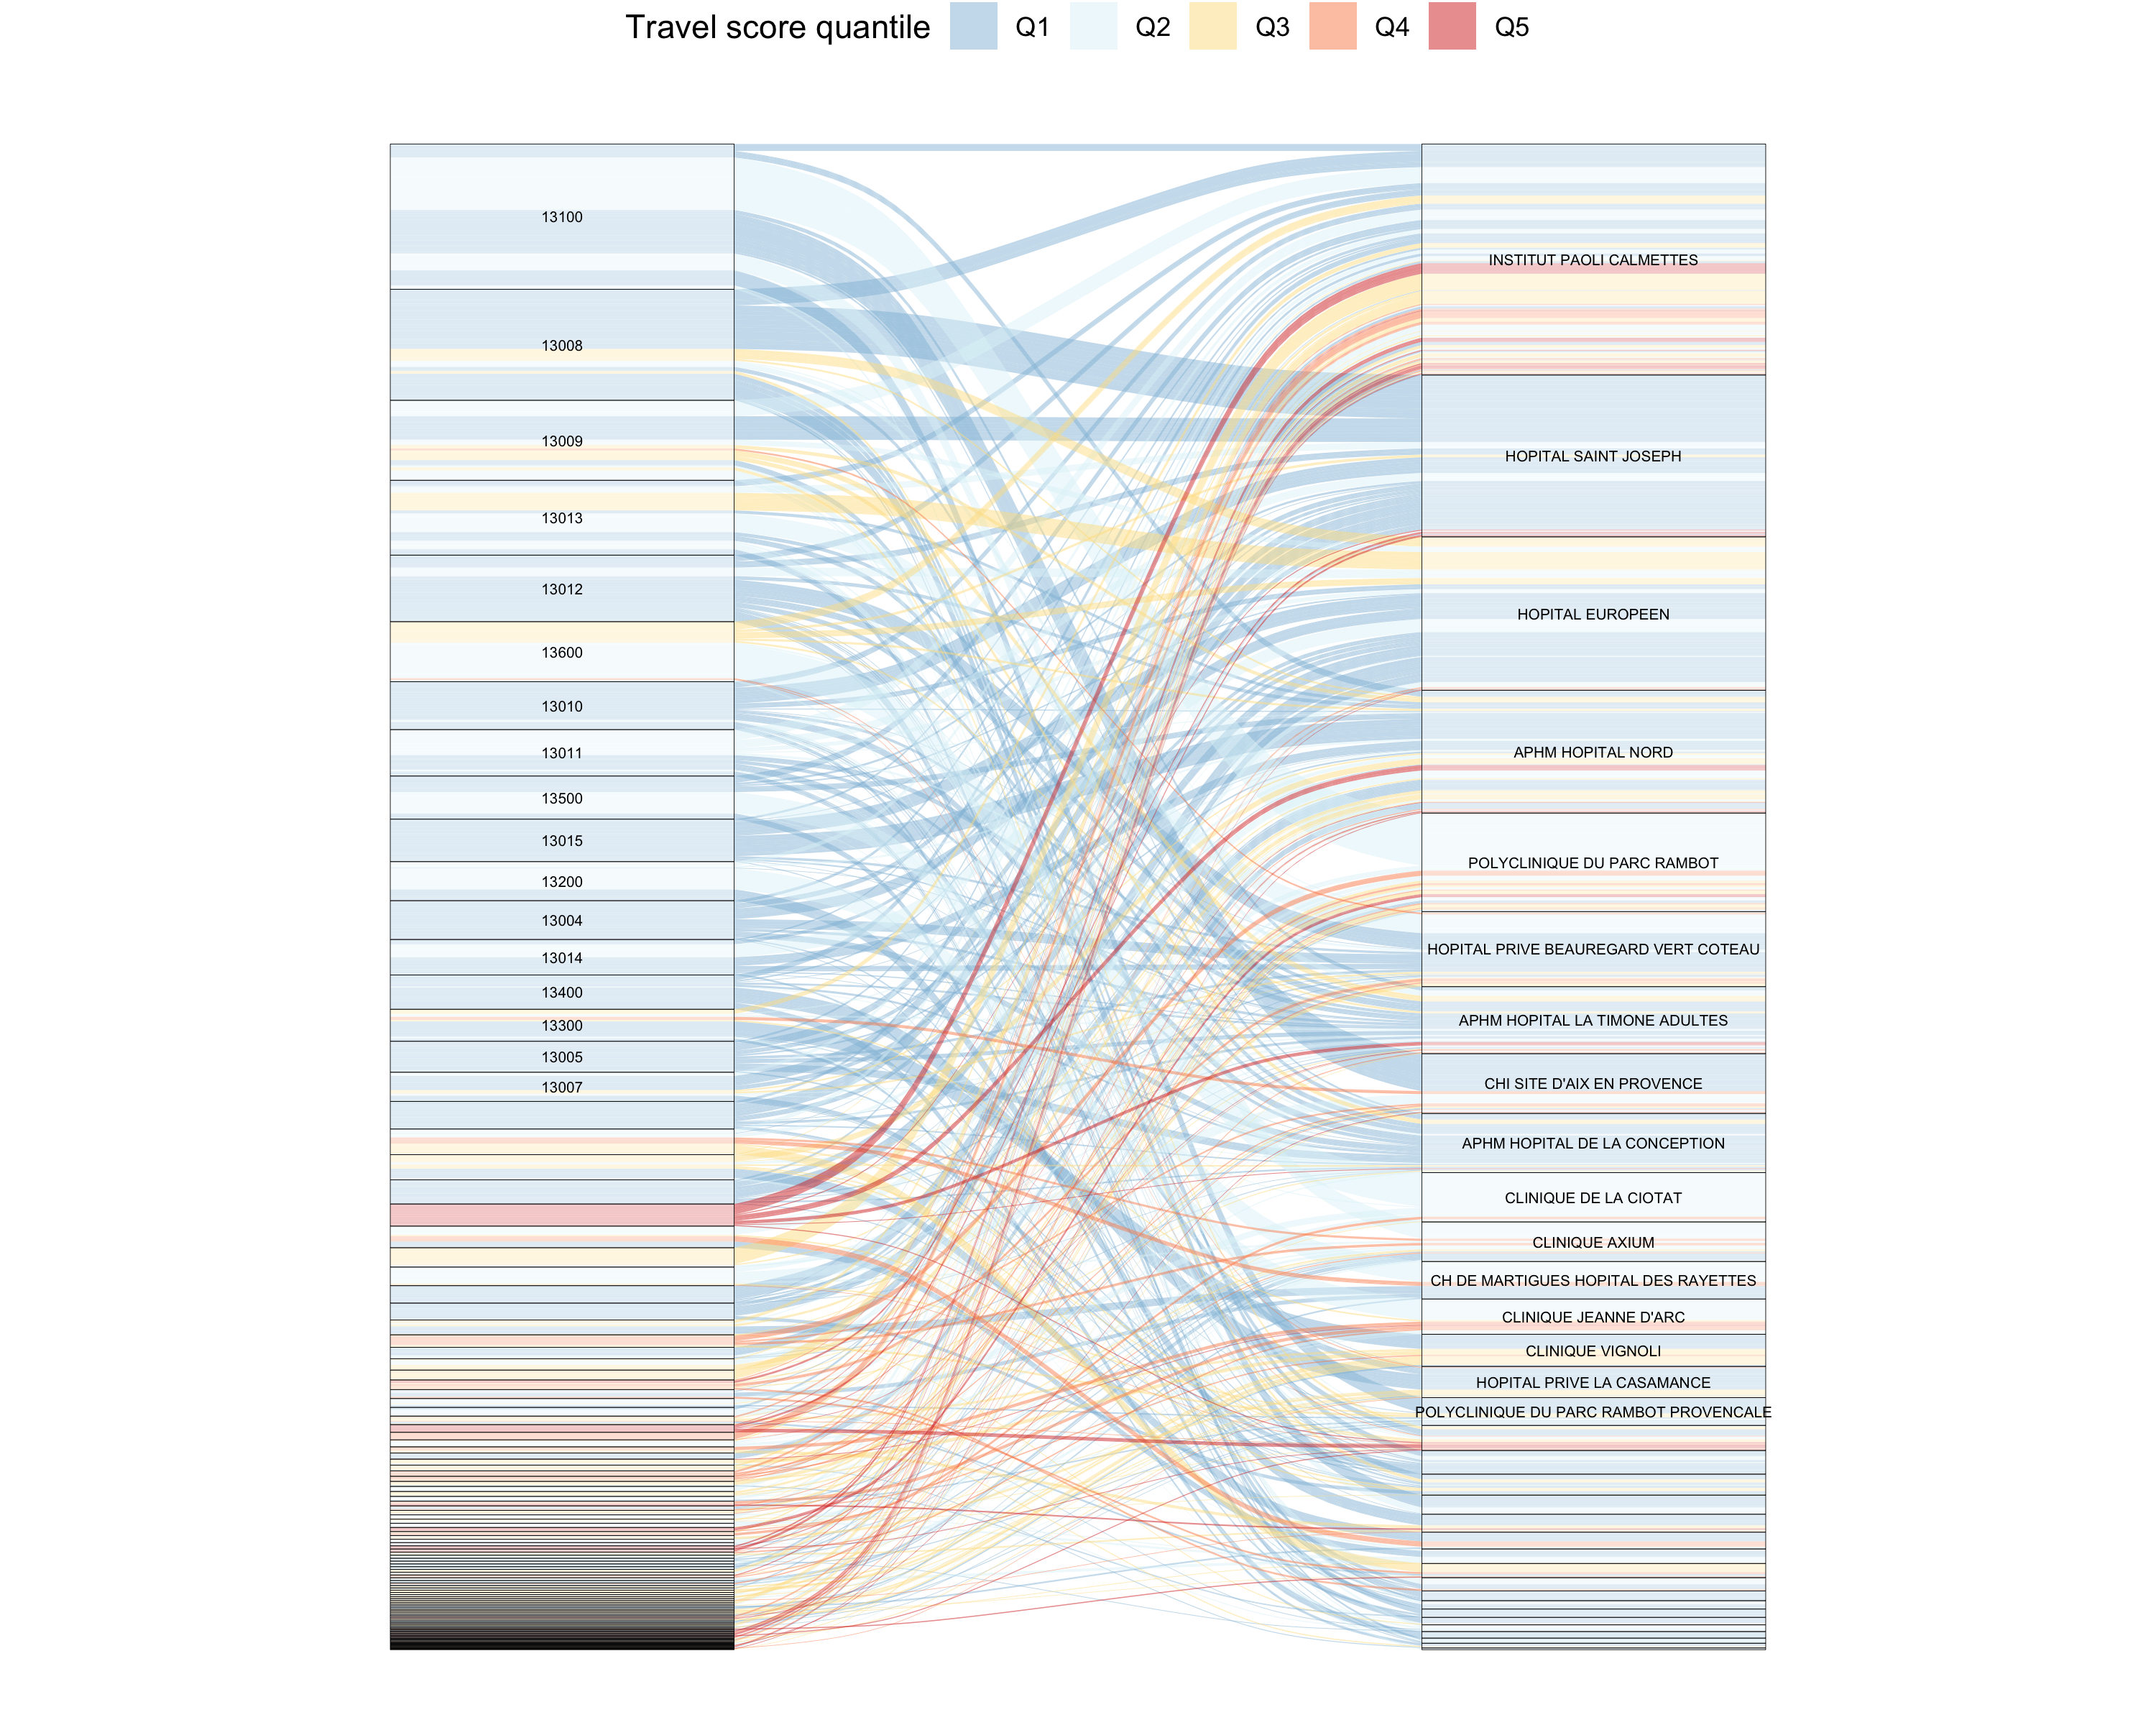
\includegraphics[width=\textwidth]{images/routes/fig6.png}
    \centering
    \caption{
        \textbf{Distribution of patients traveling to care centers located in Bouches-du-Rhone department.} Municipalities are displayed on the right side of the alluvial plot, and care centers on the left side. Municipalities are sized by the number of residing patients. Care centers are sized by the number of treated patients. Flows represent patients travel and are sized by the number of patients traveling from a municipality to a care center. The flows are colored based on the travel score quantile. We can easily identify that the patients living in smaller municipalities are more likely to experience tedious travel. Larger care centers often receive patients from these smaller municipalities.
    }
    \label{fig:routes-alluvial-13}
\end{figure}

\begin{figure}[H]
    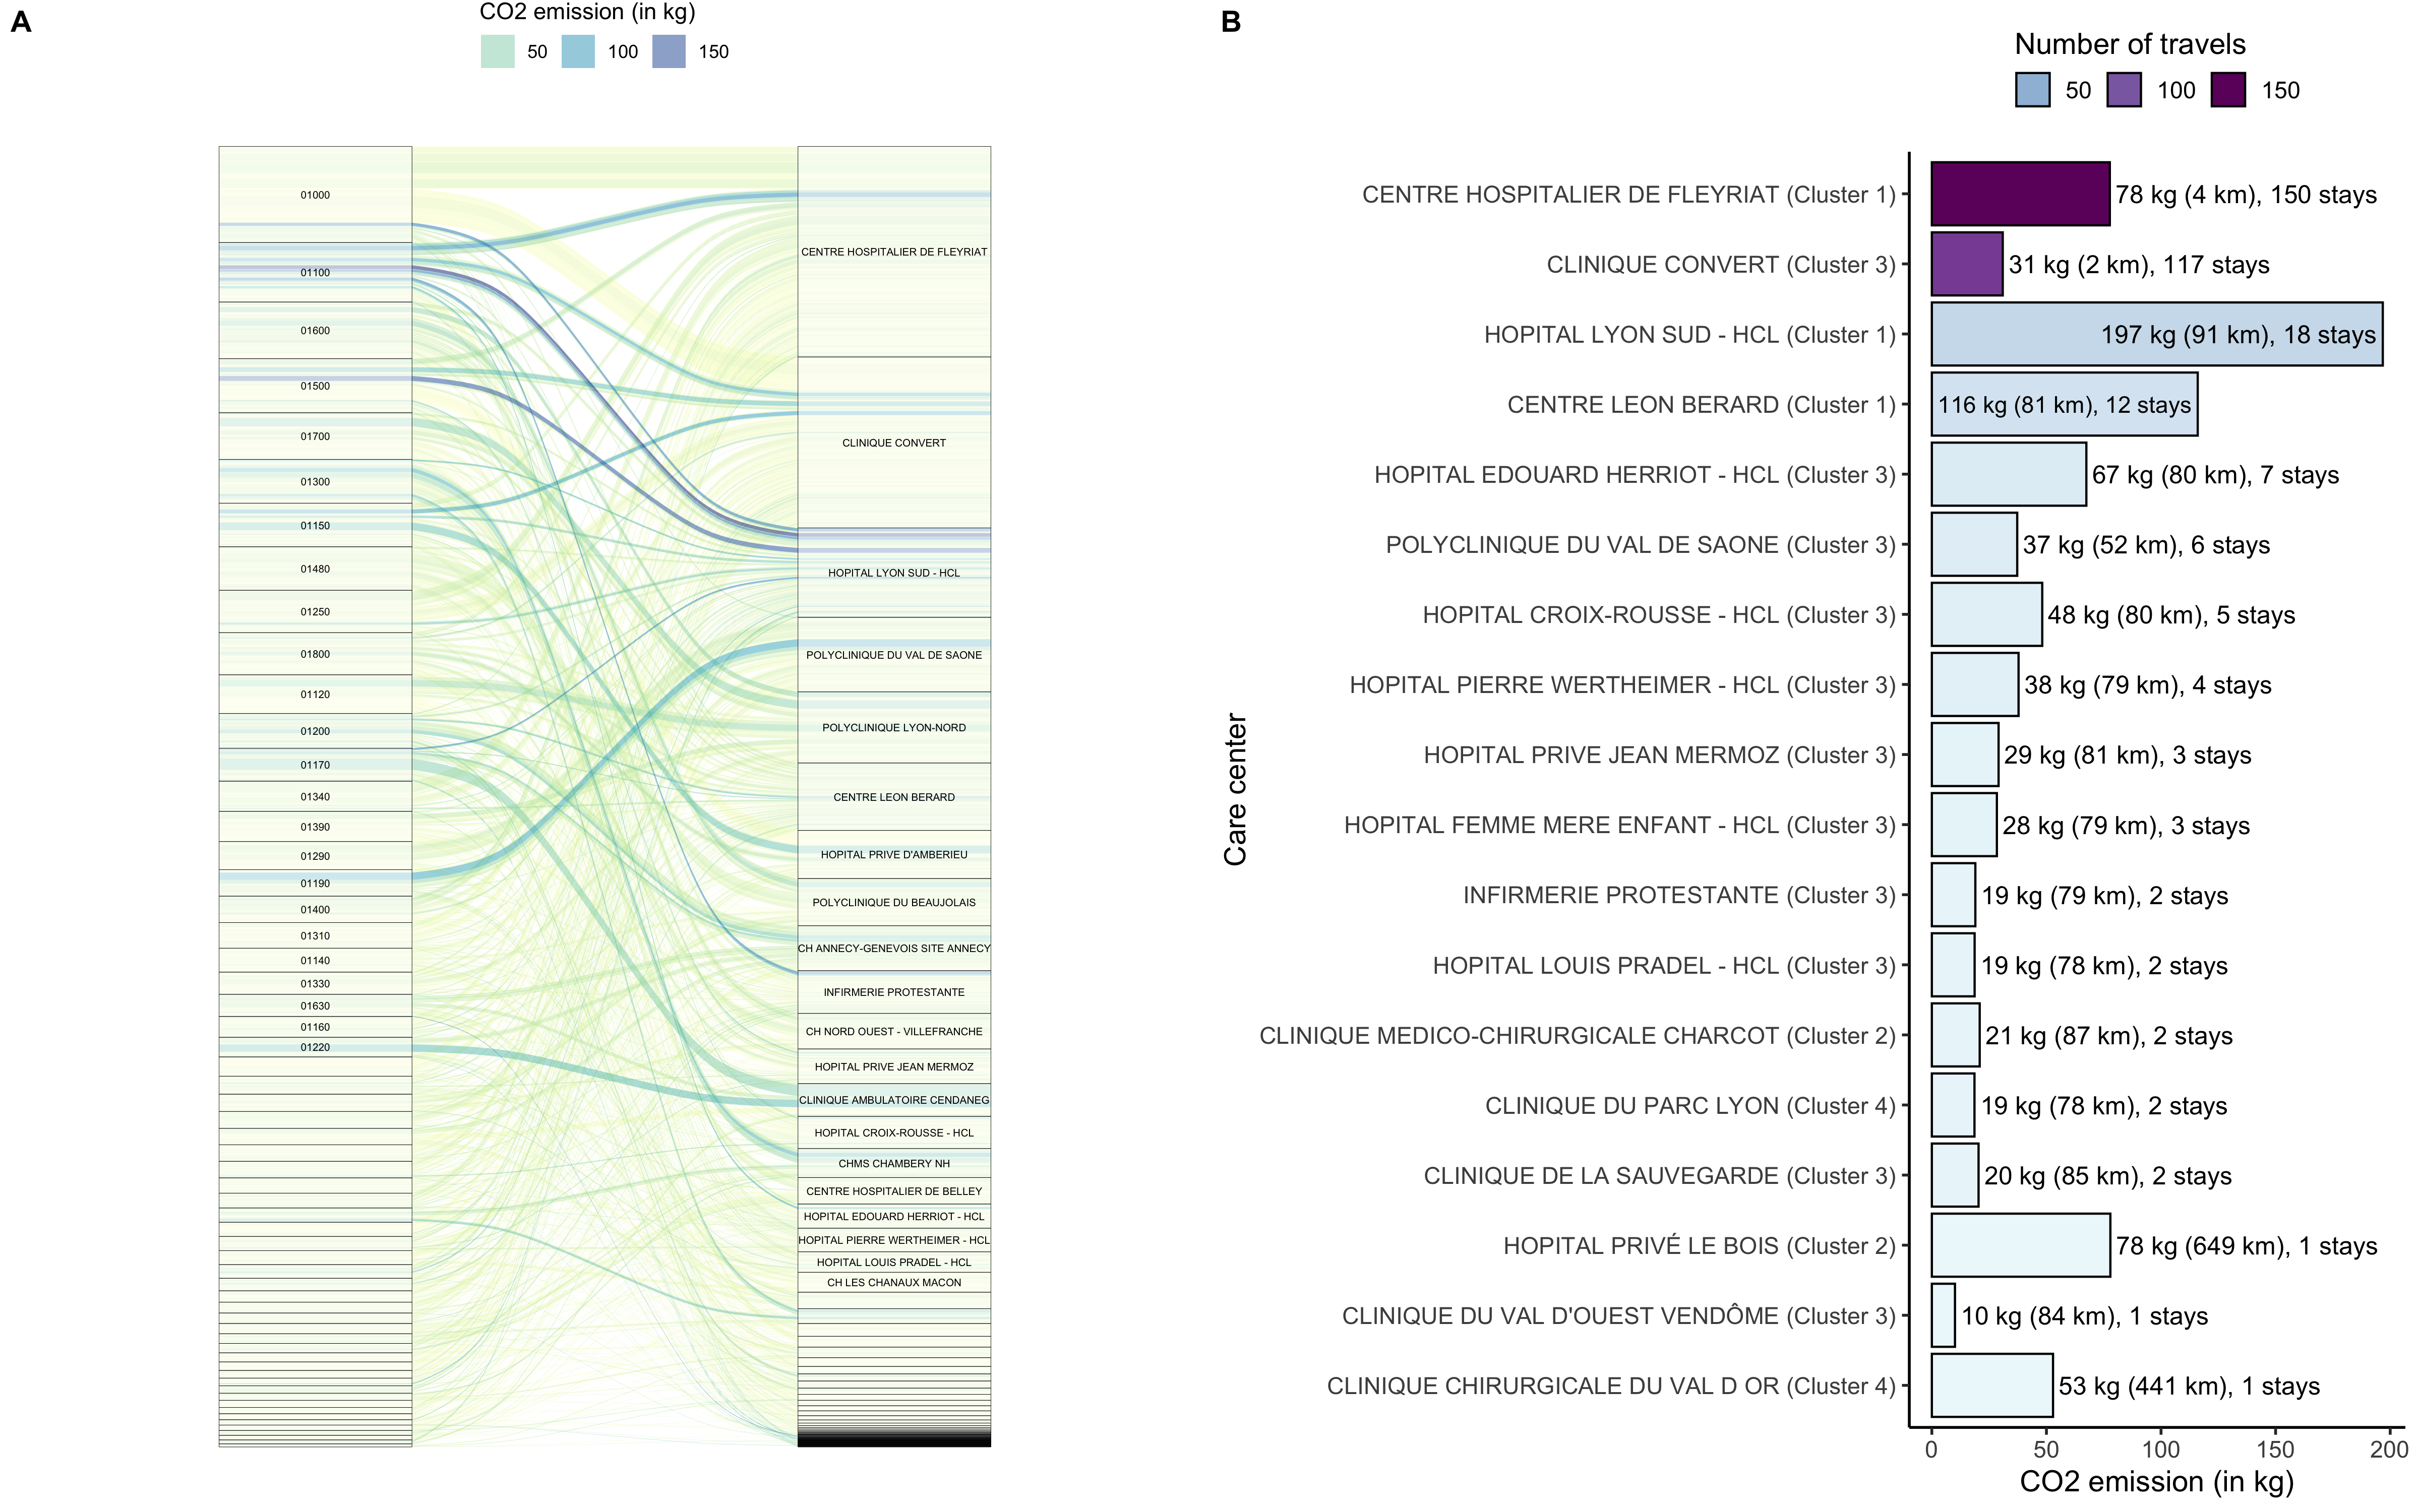
\includegraphics[width=\textwidth]{images/routes/fig8.png}
    \centering
    \caption{
        \textbf{Patients travel, sized by number of travels, and colored by \ac{co2} emission.} We study the patients travel in Bourg-en-Bresse area, a sub-urban and rural area located in Auvergne-Rhone-Alpes region. Plot (A) displays the patients flows from municipalities on the right to care centers on the left. The flows are colored by the resulting \ac{co2} emissions. \ac{co2} emissions are calculated by multiplying the travel distance by the number of travels and the car average consumption. We can see that the higher \ac{co2} emissions are not issued by travels with lots of patients, but instead from travels with fewer patients but much longer drives. This is emphasized on plot (B), showing the \ac{co2} emissions resulting from patients living in Bourg en Bresse area. Indeed, the 42 travels to Hopital Lyon Sud emitted three times as much \ac{co2} than the 253 travels to Centre Hospitalier de Fleyriat.
    }
    \label{fig:routes-co2-01}
\end{figure}

\include{chapters/5-simca}
\chapter{Side projects}

\section{Healthcare-Network}

\begin{figure}[H]
    \includegraphics[width=0.7\textwidth]{images/healthcare-network/home.png}
    \centering
    \caption{
        Healthcare-Network: homepage. A minimalist page with a search bar allowing to find hospitals based on their name, category, or location.
    }
    \label{fig:hn-home}
\end{figure}


\begin{figure}[H]
    \includegraphics[width=0.7\textwidth]{images/healthcare-network/search.png}
    \centering
    \caption{
        Healthcare-Network: search results. The list of retrieved hospitals and their details is displayed, as their position on a map. This query shows all the \ac{chru} hospitals in metropolitan France.
    }
    \label{fig:hn-search}
\end{figure}


\begin{figure}[H]
    \includegraphics[width=0.7\textwidth]{images/healthcare-network/curie-services.png}
    \centering
    \caption{
        Healthcare-Network: description of health services offered, and statistics on \ac{mco} activity for Institut Curie Paris hospital.
    }
    \label{fig:hn-curie-services}
\end{figure}


\begin{figure}[H]
    \includegraphics[width=0.7\textwidth]{images/healthcare-network/curie-cancero.png}
    \centering
    \caption{
        Healthcare-Network: description of oncology activity for Institut Curie Paris hospital.
    }
    \label{fig:hn-curie-cancero}
\end{figure}


\begin{figure}[H]
    \includegraphics[width=0.7\textwidth]{images/healthcare-network/curie-dp.png}
    \centering
    \caption{
        Healthcare-Network: number of patients per cancer related diagnosis for Institut Curie Paris hospital. Comparison with the median statistics from hospitals within the same category (\ac{clcc}) and overall median.
    }
    \label{fig:hn-curie-dp}
\end{figure}


\begin{figure}[H]
    \includegraphics[width=0.7\textwidth]{images/healthcare-network/curie-co-occ.png}
    \centering
    \caption{
        Healthcare-Network: map of the hospitals that have the most co-occurrences with Institut Curie Paris. Co-occurrences between two hospitals are defined as the number of patients who visited both hospitals during their care pathways. To illustrate facility attractiveness, municipalities are colored by the number of inhabitants who visited the Institut Curie Paris hospital.
    }
    \label{fig:hn-curie-co-occ}
\end{figure}


\begin{figure}[H]
    \includegraphics[width=0.7\textwidth]{images/healthcare-network/curie-commune.png}
    \centering
    \caption{
        Healthcare-Network: statistics on the municipality where Institut Curie Paris is located (Paris 75105). Population, median salary and accessibility to primary care are displayed to qualify the hospital neighborhood. Health professionals within the department are also listed to illustrate the health supply available around the hospital.
    }
    \label{fig:hn-curie-commune}
\end{figure}


\section{Affiliation Generator}

Affiliation Generator is a web application that helps you manage your papers authors and their affiliations. The app will let you upload a list of researchers from your team, as well as their affiliations. When you're writing a new paper, simply drag and drop authors in the required order of authorship and the app will generate the list of authors to copy-paste in your paper.

You can edit your researchers and institutions list. Every researcher can be attached to one or many institutions. The generator page will let you drag and drop researchers in the order of authorship on your paper. Once your click generate, the app will retrieve the affiliations from your researchers and format them automatically for you so that you only have to copy paste this into your paper. You can also create papers, drag and drop the authors in the order you want, save them and add more authors later.

The application is deployed within Institut Curie at the following address:

\url{https://affiliation-generator.curie.net/}.

\chapter*{Conclusion}
\addcontentsline{toc}{chapter}{Conclusion}

\subsection*{Contributions}

We recall that the purpose of this thesis was to study the geographical
and socio-demographic disparities in oncology care pathways, in
metropolitan France.

In the first chapter, we described the hospitals
available in the country, and characterized them regarding oncology
specialization. That characterization process was automatically performed
through an unsupervised clustering algorithm, trained on hospitals statistics
from the \ac{sae} public survey. We were then able to differentiate the
most suited hospitals for oncology care, and isolate the hospitals that had
no oncology activity. Then, we studied the collaborations between these
hospitals, measured by the number of patients who visited a common hospital
during their pathways. From this collaboration dataset, we could discover
communities of hospitals that frequently exchange patients together. These
communities contain hospitals with different degree of oncology specialization.
This information could be a starting point to creating oncology collaboration
groups, consisting in hospitals working together to make sure the hospitals
with less expertise are continuously trained by more specialized hospitals.

In the next chapter, we studied the accessibility to oncology care centers in
metropolitan France. We computed an accessibility score for every municipality
in metropolitan France. The score reflects how easy it would be for patients
from a given municipality to reach an oncology specialized hospital. This score
is based on a weighting between supply and demand, as well as travel impedance.
We described the spatial distribution of this score, which was higher in dense
areas, near the most specialized hospitals, identified through the clustering
step.

Then, we proposed an optimization algorithm to identify which hospitals to grow
in order to maximize the oncology accessibility. This algorithm took as input
the current accessibility distribution, as well as some user-defined
constraints. Such constraints may include a maximum hospital growth percentage,
based on the current hospital oncology specialization. Through this optimization
process, we identified a list of hospitals that should be grown in priority to
improve the oncology accessibility distribution. The results were detailed for
every region. We packaged our method into a web application, that could be used
by healthcare professionals to run simulations and eventually improve the
healthcare planning, benefiting millions of patients.

The previous work on oncology accessibility did not directly studied the actual
cancer patients routes. In the next chapter, we extracted all the visited
hospitals during the pathways of cancer patients, and described the duration and
distance traveled based on the patients residence. These results validated our
oncology accessibility score since travel durations were longer in areas with
low accessibility scores. Longer travels were shown to have a negative impact on
the patients prognosis and treatment. Moreover, long travels often increases
patients fatigue, due to the travel burden. We argued that travel duration was
not the only factor to consider when studying the tediousness of a journey. We
built a composite indicator to reflect the travel burden of a route, based on
duration, distance and road sinuosity. We showed that patients living in rural
areas had higher travel burden, due to the longer drives they experienced, as
well as the lower road quality and higher sinuosity. Finally, we proposed an
algorithm that simulates a setup where every patient would visit the closest
specialized hospital, while making sure the hospitals capacities were not
exceeded. We showed that this approach could reduce the average driving
duration by 36\%, as well as the associated carbon footprint of the journey.

Although, in practice, patients are oriented to an hospital by their general
practitioner. There are multiple evidences in the literature that patients
are not satisfied with the level of information they receive during their
pathways. In cancer care, some patients could be sent to the wrong hospital,
without them noticing. When that is the case, the hospital could either be
a well suited hospital, but unnecessarily far from the patient residence;
or an hospital that is not experienced enough in the patients pathology. For
these reasons, we built ``healthcare-network'', a web application that lists
all the hospitals in metropolitan France, and displays key statistics on them.
The application could be used by patients to learn more about the hospitals
around them, and by health professionals, to make sure the hospital they are
sending their patients are well suited for their pathologies. We believe such
tool could incentivize physicians to send patients closer to their location
of residence. Moreover, bringing more transparency to oncology care could be
a way to reduce disparities, provided that all the population has an equal
access to these online tools.

\subsection*{Future work}

Our oncology specialization clusters could be used in further research to assess
whether the oncology care pathways are more often degraded in hospitals from the
least specialized clusters. For instance, our clusters could be the input
variables of survival analyses, to assess whether there are significant
variations in the prognosis based on the oncology specialization of the chosen
hospital. More research could also be done on the effectiveness of
collaborations between the oncology communities we discovered. These communities
are a first proposition of hospitals candidates that could work together to
better treat patients in the neighboring municipalities. Similarly, our
accessibility scores could be used in survival analyses, to assess whether
patients living in the areas with low accessibility scores have more degraded
pathways and lower prognosis. Regarding the web applications we developed,
they could be introduced to healthcare professionals in France, like the
Regional Health Agencies (ARS), responsible of the organization and the
coordination of the hospitals in the country. Working closely with these
professionals would allow to adapt our tools to their needs, so they can
eventually be used in practice to take concrete decisions on the planning of
care in the country.

\end{singlespace}

%**********************
%***** References *****
%**********************

\newgeometry{top=4cm, bottom=4cm, left=2cm, right=2cm}
\bibliographystyle{vancouver}
\bibliography{references}

%%%%%%%%%%%%%%%%%%%%%%%%%%%%%%%%%%%%%%%%%%%%%%%%%%%%%%%%%%%%%%%
% 4eme de couverture
%%%%%%%%%%%%%%%%%%%%%%%%%%%%%%%%%%%%%%%%%%%%%%%%%%%%%%%%%%%%%%%

\checkoddpage
\ifoddpage \newpage\thispagestyle{empty}\null\newpage \fi

\thispagestyle{empty}
\newgeometry{top=1.5cm, bottom=1.25cm, left=2cm, right=2cm}
\fontfamily{rm}\selectfont

\lhead{}
\rhead{}
\rfoot{}
\cfoot{}
\lfoot{}

\noindent

\includegraphics[height=2.45cm]{images/logos/logo_usp_CBMS.png}
\vspace{1cm}

\fontfamily{cmss}\fontseries{m}\selectfont

\small

\input{abstract-fr}

\vspace{8mm}

\input{abstract-en}

%%%%%%%%%%%%%%%%%%%%%%%%%%
% Section headers format %
%%%%%%%%%%%%%%%%%%%%%%%%%%

\titleformat{\chapter}[hang]{\bfseries\Large\color{Prune}}{\thechapter\ -}{.1ex}
{\vspace{0.1ex}
}
[\vspace{1ex}]
\titlespacing{\chapter}{0pc}{0ex}{0.5pc}

\titleformat{\section}[hang]{\bfseries\normalsize}{\thesection\ .}{0.5pt}
{\vspace{0.1ex}
}
[\vspace{0.1ex}]
\titlespacing{\section}{1.5pc}{4ex plus .1ex minus .2ex}{.8pc}

\titleformat{\subsection}[hang]{\bfseries\small}{\thesubsection\ .}{1pt}
{\vspace{0.1ex}
}
[\vspace{0.1ex}]
\titlespacing{\subsection}{3pc}{2ex plus .1ex minus .2ex}{.1pc}

\end{document}
